% Options for packages loaded elsewhere
\PassOptionsToPackage{unicode}{hyperref}
\PassOptionsToPackage{hyphens}{url}
%
\documentclass[
]{article}
\usepackage{lmodern}
\usepackage{amssymb,amsmath}
\usepackage{ifxetex,ifluatex}
\ifnum 0\ifxetex 1\fi\ifluatex 1\fi=0 % if pdftex
  \usepackage[T1]{fontenc}
  \usepackage[utf8]{inputenc}
  \usepackage{textcomp} % provide euro and other symbols
\else % if luatex or xetex
  \usepackage{unicode-math}
  \defaultfontfeatures{Scale=MatchLowercase}
  \defaultfontfeatures[\rmfamily]{Ligatures=TeX,Scale=1}
\fi
% Use upquote if available, for straight quotes in verbatim environments
\IfFileExists{upquote.sty}{\usepackage{upquote}}{}
\IfFileExists{microtype.sty}{% use microtype if available
  \usepackage[]{microtype}
  \UseMicrotypeSet[protrusion]{basicmath} % disable protrusion for tt fonts
}{}
\makeatletter
\@ifundefined{KOMAClassName}{% if non-KOMA class
  \IfFileExists{parskip.sty}{%
    \usepackage{parskip}
  }{% else
    \setlength{\parindent}{0pt}
    \setlength{\parskip}{6pt plus 2pt minus 1pt}}
}{% if KOMA class
  \KOMAoptions{parskip=half}}
\makeatother
\usepackage{xcolor}
\IfFileExists{xurl.sty}{\usepackage{xurl}}{} % add URL line breaks if available
\IfFileExists{bookmark.sty}{\usepackage{bookmark}}{\usepackage{hyperref}}
\hypersetup{
  pdftitle={Documentation of the Payment Delays Project},
  pdfauthor={Ivana Stanova, Lenka Stastna},
  hidelinks,
  pdfcreator={LaTeX via pandoc}}
\urlstyle{same} % disable monospaced font for URLs
\usepackage[margin=1in]{geometry}
\usepackage{longtable,booktabs}
% Correct order of tables after \paragraph or \subparagraph
\usepackage{etoolbox}
\makeatletter
\patchcmd\longtable{\par}{\if@noskipsec\mbox{}\fi\par}{}{}
\makeatother
% Allow footnotes in longtable head/foot
\IfFileExists{footnotehyper.sty}{\usepackage{footnotehyper}}{\usepackage{footnote}}
\makesavenoteenv{longtable}
\usepackage{graphicx,grffile}
\makeatletter
\def\maxwidth{\ifdim\Gin@nat@width>\linewidth\linewidth\else\Gin@nat@width\fi}
\def\maxheight{\ifdim\Gin@nat@height>\textheight\textheight\else\Gin@nat@height\fi}
\makeatother
% Scale images if necessary, so that they will not overflow the page
% margins by default, and it is still possible to overwrite the defaults
% using explicit options in \includegraphics[width, height, ...]{}
\setkeys{Gin}{width=\maxwidth,height=\maxheight,keepaspectratio}
% Set default figure placement to htbp
\makeatletter
\def\fps@figure{htbp}
\makeatother
\setlength{\emergencystretch}{3em} % prevent overfull lines
\providecommand{\tightlist}{%
  \setlength{\itemsep}{0pt}\setlength{\parskip}{0pt}}
\setcounter{secnumdepth}{5}

\title{Documentation of the Payment Delays Project}
\author{Ivana Stanova, Lenka Stastna}
\date{10 1 2021}

\begin{document}
\maketitle

{
\setcounter{tocdepth}{2}
\tableofcontents
}
\hypertarget{business-understanding}{%
\section{Business Understanding}\label{business-understanding}}

The main topic of this data science project is to optimize the collection process. Sponsor of the project is Mr.~Jiří Procházka, who decided on the scope of the project, provided data and helped define project deliverables.

First of all, it was important to understand the collection process. Clients are paying a certain amount due to a certain date. If the client delays his payment, certain collection procedure takes place because of the costs that rise for the company. There are three actions taking place under different conditions. If the payment is delayed for 21 - 69 days, first action is taken. Second action is taken if the delay is between 70 - 139 days and the third action is taken for delay greater than 140 days.\\
Our goal was to create three models. First model predicts whether the customer will be delayed in payment for 21+ days. Second model predicts whether the customer will be delayed in payment for 140+ days. Lastly, third model should estimate the average number of days delayed if the client would exceed the first action. All three models were defined baseline accuracy, to which created models were compared.

As one of the deliverables, project documentation describes project flow. Project consisted of three major steps: Data preparation, Modeling, Evaluation. All of the phases are described in detail with visualized results and findings in this document.\\
We chose to use R studio to prepare the data, create models and evaluate, RMarkdown was used to create documentation of the project.

\hypertarget{data-preparation}{%
\section{Data Preparation}\label{data-preparation}}

\hypertarget{data-understanding}{%
\subsection{Data Understanding}\label{data-understanding}}

\hypertarget{data-description-report}{%
\subsubsection{Data Description Report}\label{data-description-report}}

The initial data was provided in a comma-separated values file, and was loaded and processed using the R programming language. Dataset used in this project contains 2 353 012 observations and 24 variables. Out of the 24 variables, 13 are of factor datatype, 9 are numeric and 2 are dates. All columns from the initial dataset were converted to the correct datype according to the data description file, which was provided. Column \emph{payed\_ammount} was replaced by column \emph{paid\_amount}. Column \emph{payment\_date} originally contained some blank fields, which were subsequently filled in as NA.
We also created a new feature \emph{delay} at the beginning of our work as the target variable. Variable stands for the difference between \emph{payment\_date} and \emph{due\_date}.

\begin{longtable}[]{@{}llll@{}}
\toprule
\begin{minipage}[b]{0.30\columnwidth}\raggedright
Column name\strut
\end{minipage} & \begin{minipage}[b]{0.30\columnwidth}\raggedright
Description\strut
\end{minipage} & \begin{minipage}[b]{0.11\columnwidth}\raggedright
Type\strut
\end{minipage} & \begin{minipage}[b]{0.19\columnwidth}\raggedright
Values\strut
\end{minipage}\tabularnewline
\midrule
\endhead
\begin{minipage}[t]{0.30\columnwidth}\raggedright
contract\_id\strut
\end{minipage} & \begin{minipage}[t]{0.30\columnwidth}\raggedright
Unique identificator of the contract\strut
\end{minipage} & \begin{minipage}[t]{0.11\columnwidth}\raggedright
Int\strut
\end{minipage} & \begin{minipage}[t]{0.19\columnwidth}\raggedright
\{1,2,3,\ldots,N\}\strut
\end{minipage}\tabularnewline
\begin{minipage}[t]{0.30\columnwidth}\raggedright
payment\_order\strut
\end{minipage} & \begin{minipage}[t]{0.30\columnwidth}\raggedright
Order of the payment\strut
\end{minipage} & \begin{minipage}[t]{0.11\columnwidth}\raggedright
Int\strut
\end{minipage} & \begin{minipage}[t]{0.19\columnwidth}\raggedright
\{1,2,3,\ldots\}\strut
\end{minipage}\tabularnewline
\begin{minipage}[t]{0.30\columnwidth}\raggedright
due\_date\strut
\end{minipage} & \begin{minipage}[t]{0.30\columnwidth}\raggedright
Payment deadline\strut
\end{minipage} & \begin{minipage}[t]{0.11\columnwidth}\raggedright
Date\strut
\end{minipage} & \begin{minipage}[t]{0.19\columnwidth}\raggedright
YY/MM/DD\strut
\end{minipage}\tabularnewline
\begin{minipage}[t]{0.30\columnwidth}\raggedright
payment\_date\strut
\end{minipage} & \begin{minipage}[t]{0.30\columnwidth}\raggedright
Date of the payment\strut
\end{minipage} & \begin{minipage}[t]{0.11\columnwidth}\raggedright
Date\strut
\end{minipage} & \begin{minipage}[t]{0.19\columnwidth}\raggedright
YY/MM/DD\strut
\end{minipage}\tabularnewline
\begin{minipage}[t]{0.30\columnwidth}\raggedright
product\_type\strut
\end{minipage} & \begin{minipage}[t]{0.30\columnwidth}\raggedright
Type of the product\strut
\end{minipage} & \begin{minipage}[t]{0.11\columnwidth}\raggedright
Factor\strut
\end{minipage} & \begin{minipage}[t]{0.19\columnwidth}\raggedright
\{1,2,3,4,5\}\strut
\end{minipage}\tabularnewline
\begin{minipage}[t]{0.30\columnwidth}\raggedright
contract\_status\strut
\end{minipage} & \begin{minipage}[t]{0.30\columnwidth}\raggedright
Contract status\strut
\end{minipage} & \begin{minipage}[t]{0.11\columnwidth}\raggedright
Factor\strut
\end{minipage} & \begin{minipage}[t]{0.19\columnwidth}\raggedright
\{1,2,3,4,5,6,7,8,9\}\strut
\end{minipage}\tabularnewline
\begin{minipage}[t]{0.30\columnwidth}\raggedright
business\_discount\strut
\end{minipage} & \begin{minipage}[t]{0.30\columnwidth}\raggedright
Business discount provided\strut
\end{minipage} & \begin{minipage}[t]{0.11\columnwidth}\raggedright
Factor\strut
\end{minipage} & \begin{minipage}[t]{0.19\columnwidth}\raggedright
\{0,1\}\strut
\end{minipage}\tabularnewline
\begin{minipage}[t]{0.30\columnwidth}\raggedright
gender\strut
\end{minipage} & \begin{minipage}[t]{0.30\columnwidth}\raggedright
Gender\strut
\end{minipage} & \begin{minipage}[t]{0.11\columnwidth}\raggedright
Factor\strut
\end{minipage} & \begin{minipage}[t]{0.19\columnwidth}\raggedright
\{1,2\}\strut
\end{minipage}\tabularnewline
\begin{minipage}[t]{0.30\columnwidth}\raggedright
marital\_status\strut
\end{minipage} & \begin{minipage}[t]{0.30\columnwidth}\raggedright
Marital status\strut
\end{minipage} & \begin{minipage}[t]{0.11\columnwidth}\raggedright
Factor\strut
\end{minipage} & \begin{minipage}[t]{0.19\columnwidth}\raggedright
\{1,2,3,4,5,6\}\strut
\end{minipage}\tabularnewline
\begin{minipage}[t]{0.30\columnwidth}\raggedright
number\_of\_children\strut
\end{minipage} & \begin{minipage}[t]{0.30\columnwidth}\raggedright
Number of children\strut
\end{minipage} & \begin{minipage}[t]{0.11\columnwidth}\raggedright
Int\strut
\end{minipage} & \begin{minipage}[t]{0.19\columnwidth}\raggedright
\{1,2,3,\ldots\}\strut
\end{minipage}\tabularnewline
\begin{minipage}[t]{0.30\columnwidth}\raggedright
number\_other\_product\strut
\end{minipage} & \begin{minipage}[t]{0.30\columnwidth}\raggedright
Number of other products\strut
\end{minipage} & \begin{minipage}[t]{0.11\columnwidth}\raggedright
Int\strut
\end{minipage} & \begin{minipage}[t]{0.19\columnwidth}\raggedright
\{1,2,3,\ldots\}\strut
\end{minipage}\tabularnewline
\begin{minipage}[t]{0.30\columnwidth}\raggedright
clients\_phone\strut
\end{minipage} & \begin{minipage}[t]{0.30\columnwidth}\raggedright
T/F if the client filled in home phone\strut
\end{minipage} & \begin{minipage}[t]{0.11\columnwidth}\raggedright
Factor\strut
\end{minipage} & \begin{minipage}[t]{0.19\columnwidth}\raggedright
\{True, False\}\strut
\end{minipage}\tabularnewline
\begin{minipage}[t]{0.30\columnwidth}\raggedright
client\_mobile\strut
\end{minipage} & \begin{minipage}[t]{0.30\columnwidth}\raggedright
T/F if the client filled in mobile phone\strut
\end{minipage} & \begin{minipage}[t]{0.11\columnwidth}\raggedright
Factor\strut
\end{minipage} & \begin{minipage}[t]{0.19\columnwidth}\raggedright
\{True, False\}\strut
\end{minipage}\tabularnewline
\begin{minipage}[t]{0.30\columnwidth}\raggedright
client\_email\strut
\end{minipage} & \begin{minipage}[t]{0.30\columnwidth}\raggedright
T/F if the client filled in email address\strut
\end{minipage} & \begin{minipage}[t]{0.11\columnwidth}\raggedright
Factor\strut
\end{minipage} & \begin{minipage}[t]{0.19\columnwidth}\raggedright
\{True, False\}\strut
\end{minipage}\tabularnewline
\begin{minipage}[t]{0.30\columnwidth}\raggedright
total\_earnings\strut
\end{minipage} & \begin{minipage}[t]{0.30\columnwidth}\raggedright
Earning bucket\strut
\end{minipage} & \begin{minipage}[t]{0.11\columnwidth}\raggedright
Factor\strut
\end{minipage} & \begin{minipage}[t]{0.19\columnwidth}\raggedright
\{level1,\ldots, not\_declared\}\strut
\end{minipage}\tabularnewline
\begin{minipage}[t]{0.30\columnwidth}\raggedright
birth\_year\strut
\end{minipage} & \begin{minipage}[t]{0.30\columnwidth}\raggedright
Birth year of the client\strut
\end{minipage} & \begin{minipage}[t]{0.11\columnwidth}\raggedright
Int\strut
\end{minipage} & \begin{minipage}[t]{0.19\columnwidth}\raggedright
\{1990,1991,\ldots\}\strut
\end{minipage}\tabularnewline
\begin{minipage}[t]{0.30\columnwidth}\raggedright
birth\_month\strut
\end{minipage} & \begin{minipage}[t]{0.30\columnwidth}\raggedright
Birth month of the client\strut
\end{minipage} & \begin{minipage}[t]{0.11\columnwidth}\raggedright
Int\strut
\end{minipage} & \begin{minipage}[t]{0.19\columnwidth}\raggedright
\{1,2,3,\ldots\}\strut
\end{minipage}\tabularnewline
\begin{minipage}[t]{0.30\columnwidth}\raggedright
living\_area\strut
\end{minipage} & \begin{minipage}[t]{0.30\columnwidth}\raggedright
Region of the client home address\strut
\end{minipage} & \begin{minipage}[t]{0.11\columnwidth}\raggedright
Factor\strut
\end{minipage} & \begin{minipage}[t]{0.19\columnwidth}\raggedright
\{1,2,3,\ldots\}\strut
\end{minipage}\tabularnewline
\begin{minipage}[t]{0.30\columnwidth}\raggedright
different\_contact\_area\strut
\end{minipage} & \begin{minipage}[t]{0.30\columnwidth}\raggedright
T/F if the client filled different home and contact address\strut
\end{minipage} & \begin{minipage}[t]{0.11\columnwidth}\raggedright
Factor\strut
\end{minipage} & \begin{minipage}[t]{0.19\columnwidth}\raggedright
\{True, False\}\strut
\end{minipage}\tabularnewline
\begin{minipage}[t]{0.30\columnwidth}\raggedright
kc\_flag\strut
\end{minipage} & \begin{minipage}[t]{0.30\columnwidth}\raggedright
T/F if the client does not home local citizenship\strut
\end{minipage} & \begin{minipage}[t]{0.11\columnwidth}\raggedright
Factor\strut
\end{minipage} & \begin{minipage}[t]{0.19\columnwidth}\raggedright
\{True, False\}\strut
\end{minipage}\tabularnewline
\begin{minipage}[t]{0.30\columnwidth}\raggedright
cf\_val\strut
\end{minipage} & \begin{minipage}[t]{0.30\columnwidth}\raggedright
If the special measure during the underwriting was applied\strut
\end{minipage} & \begin{minipage}[t]{0.11\columnwidth}\raggedright
Numeric\strut
\end{minipage} & \begin{minipage}[t]{0.19\columnwidth}\raggedright
\{-N,\ldots,N\}\strut
\end{minipage}\tabularnewline
\begin{minipage}[t]{0.30\columnwidth}\raggedright
kzmz\_flag\strut
\end{minipage} & \begin{minipage}[t]{0.30\columnwidth}\raggedright
T/F if the client filled in employer\strut
\end{minipage} & \begin{minipage}[t]{0.11\columnwidth}\raggedright
Factor\strut
\end{minipage} & \begin{minipage}[t]{0.19\columnwidth}\raggedright
\{True, False\}\strut
\end{minipage}\tabularnewline
\begin{minipage}[t]{0.30\columnwidth}\raggedright
due\_amount\strut
\end{minipage} & \begin{minipage}[t]{0.30\columnwidth}\raggedright
Installment what should be payed\strut
\end{minipage} & \begin{minipage}[t]{0.11\columnwidth}\raggedright
Numeric\strut
\end{minipage} & \begin{minipage}[t]{0.19\columnwidth}\raggedright
(0,\ldots)\strut
\end{minipage}\tabularnewline
\begin{minipage}[t]{0.30\columnwidth}\raggedright
payed\_amount\strut
\end{minipage} & \begin{minipage}[t]{0.30\columnwidth}\raggedright
What was payed at a certain date\strut
\end{minipage} & \begin{minipage}[t]{0.11\columnwidth}\raggedright
Numeric\strut
\end{minipage} & \begin{minipage}[t]{0.19\columnwidth}\raggedright
(0,\ldots)\strut
\end{minipage}\tabularnewline
\begin{minipage}[t]{0.30\columnwidth}\raggedright
delay\strut
\end{minipage} & \begin{minipage}[t]{0.30\columnwidth}\raggedright
Difference between payment\_date and due\_date\strut
\end{minipage} & \begin{minipage}[t]{0.11\columnwidth}\raggedright
Int\strut
\end{minipage} & \begin{minipage}[t]{0.19\columnwidth}\raggedright
\{-N,\ldots,N\}\strut
\end{minipage}\tabularnewline
\bottomrule
\end{longtable}

\hypertarget{attribute-correlations}{%
\subsubsection{Attribute correlations}\label{attribute-correlations}}

We computed correlation coefficients between all possible pairs of numeric variables, see Figure \ref{fig:correlogram}, and discovered strong positive correlation between \emph{due amount} and \emph{paid amount}. This could be due to the fact that in the event that the installment has already been paid, the due amount and the paid amount would assume the same value. Correlation between the remaining pairs of numeric variables was either nonexistent or negligible.\\
Then, the significance of correlation between due amount and paid amount was tested using Pearson's product moment correlation coefficient. The pair of attributes was found to be significantly correlated with a correlation coefficient of 0.76 and p-value less than 2.2e-16.\\
Relationship between categorical variables was tested using chi-squared test with the significance level of 0.05. All significantly correlated pairs of variables can be accessed in ``categorical\_rel'' dataframe.

\hypertarget{basic-statistics}{%
\subsubsection{Basic statistics}\label{basic-statistics}}

Basic statistics computed for numeric variables can be located in Table \ref{tab:Stats}. Frequency, relative frequency and relative cumulative frequency were computed for each categorical variable and its categories. All frequency tables can be located in the ``frequencies'' list.

\hypertarget{data-exploration-report}{%
\subsection{Data Exploration Report}\label{data-exploration-report}}

Distribution of numeric and categorical variables was visualized using boxplots, density plots and histograms, see Figure \ref{fig:density} and Figure \ref{fig:boxplots}. Next, we performed bivariate analysis of continuous variables with respect to categorical variables on selected pairs of features. The results for depedence on gender can be accessed in tables ``data\_GPA'' (dependence of paid amount on gender), ``data\_GD'' (Statistical dependence of delay on gender), ``data\_GDA'' (Statistical dependence of due amount on gender). We found out that business discount applies only to product type 1, as seen in Figure \ref{fig:delay-gender-prod}. Product type 1 displayed the highest median delay at around 25 days, followed by products 2, 3, 4, all with median delay at around 10 days. Product type 5 displayed the lowest median delay. The results did not significantly differ between the genders.

\hypertarget{data-quality-report}{%
\subsection{Data Quality Report}\label{data-quality-report}}

\hypertarget{data-coverage}{%
\subsubsection{Data coverage}\label{data-coverage}}

Next step consisted of the data coverage and plausibility analysis.\\
We did not find the results surprising, but as an example, we have chosen a couple of plots, that indicate interesting data distribution. We, for example, found out that clients mostly order the product type 1, contracts are mostly in status 5 or that most of the payments have a discount. We also discovered, that the marital status of the clients is mostly number 3 and they have most frequently no children. Clients also very frequently do not provide information about their earnings and they usually ordered 1 other product. Although the distribution of values across factor variables is not even, we do not think, the findings have to be analyzed closely.All the mentioned findings can be seen on visualizations in Figure \ref{fig:distribution}.

\hypertarget{missing-values}{%
\subsubsection{Missing values}\label{missing-values}}

Exploring the NA values in the dataset, we found out, that 4 attributes had
almost the same percentage of missing values, as can be seen in the statistics \ref{tab:Missing-stat}.\\
Attributes \emph{kc\_flag}, \emph{living\_area}, \emph{cf\_val} and \emph{different\_contact\_area} have the most missing values, almost 20 \%, whereas \emph{payment\_order} has around 3,5 \% and \emph{payment\_date} and \emph{delay} have the same percentage, almost 0,5 \%.\\
Using a different visualization, that can be seen in Figure \ref{fig:Missing-complex} or Figure \ref{fig:missing-H}, we discovered, that the four attributes with the highest percentage are
not missing at random but almost all at the same time.\\
We found out, that contract\_id together with payment\_order were not creating a unique key of the payment. One payment was divided into multiple parts, which was also causing problem with NA values in the four attributes. Data in the four attributes were not copied into other parts of a payment, but were present in just the first payment part.\\
We decided to unify the payment parts into only one payment by summarizing the paid amount of all the parts and using the payment\_date of the last paid part. Thanks to the unification, the amount of NA values has markedly decreased.\\
Secondly, we dealt with the NA values in payment\_order and payment\_date. Since it was only less then 4 \% of the dataset, and it was not possible to substitute the values, we decided to delete the rows.

\hypertarget{feature-engineering}{%
\subsection{Feature engineering}\label{feature-engineering}}

We decided to add new features to create higher-accuracy models. As already have been mentioned, we firstly computed a numeric feature \emph{delay} counting the difference of days between \emph{payment\_date} and \emph{due\_date}. We selected this variable as our target variable.

Since we are creating two classification models deciding whether a new payment will be delayed
for more than 21 days or more than 140 days, we created 2 new factor features \emph{delay\_21\_y} and \emph{delay\_140\_y}. Value is set to 1 if the payment delay is greater than 21 or greater than 140 days.

We also created a new numerical feature \emph{delay\_indiv} counting the mean delay for the whole client´s history. We also computed 2 new numerical features, \emph{delay\_indiv\_21} and \emph{delay\_indiv\_140} counting number of delayed payments (21, 140 days) for the whole client's history.

Lastly, numerical features \emph{mean\_delay\_1m} ,\emph{mean\_delay\_3m}, \emph{mean\_delay\_6m}, \emph{mean\_delay\_12m} are computing the mean delay for the last 1/3/6/12 months in the client´s history.

\hypertarget{exploratory-analysis-of-the-new-features}{%
\subsection{Exploratory analysis of the new features}\label{exploratory-analysis-of-the-new-features}}

Adding new variables, we started to work with 34 variables. We created
2 factor variables and 8 numerical variables

\hypertarget{data-description-report-1}{%
\subsubsection{Data description report}\label{data-description-report-1}}

\begin{longtable}[]{@{}llll@{}}
\toprule
\begin{minipage}[b]{0.30\columnwidth}\raggedright
Column name\strut
\end{minipage} & \begin{minipage}[b]{0.30\columnwidth}\raggedright
Description\strut
\end{minipage} & \begin{minipage}[b]{0.11\columnwidth}\raggedright
Type\strut
\end{minipage} & \begin{minipage}[b]{0.19\columnwidth}\raggedright
Values\strut
\end{minipage}\tabularnewline
\midrule
\endhead
\begin{minipage}[t]{0.30\columnwidth}\raggedright
delay\_21\_y\strut
\end{minipage} & \begin{minipage}[t]{0.30\columnwidth}\raggedright
T/F if the delay is more than 21 days\strut
\end{minipage} & \begin{minipage}[t]{0.11\columnwidth}\raggedright
Factor\strut
\end{minipage} & \begin{minipage}[t]{0.19\columnwidth}\raggedright
\{True, False\}\strut
\end{minipage}\tabularnewline
\begin{minipage}[t]{0.30\columnwidth}\raggedright
delay\_140\_y\strut
\end{minipage} & \begin{minipage}[t]{0.30\columnwidth}\raggedright
T/F if the delay is more than 140 days\strut
\end{minipage} & \begin{minipage}[t]{0.11\columnwidth}\raggedright
Factor\strut
\end{minipage} & \begin{minipage}[t]{0.19\columnwidth}\raggedright
\{True, False\}\strut
\end{minipage}\tabularnewline
\begin{minipage}[t]{0.30\columnwidth}\raggedright
delay\_indiv\strut
\end{minipage} & \begin{minipage}[t]{0.30\columnwidth}\raggedright
Mean delay for the whole client's history\strut
\end{minipage} & \begin{minipage}[t]{0.11\columnwidth}\raggedright
Int\strut
\end{minipage} & \begin{minipage}[t]{0.19\columnwidth}\raggedright
\{-N,\ldots,N\}\strut
\end{minipage}\tabularnewline
\begin{minipage}[t]{0.30\columnwidth}\raggedright
delay\_indiv\_21\strut
\end{minipage} & \begin{minipage}[t]{0.30\columnwidth}\raggedright
Cumulative sum of payments delayed for more than 21 days by contract\strut
\end{minipage} & \begin{minipage}[t]{0.11\columnwidth}\raggedright
Int\strut
\end{minipage} & \begin{minipage}[t]{0.19\columnwidth}\raggedright
\{1,2,3,\ldots,N\}\strut
\end{minipage}\tabularnewline
\begin{minipage}[t]{0.30\columnwidth}\raggedright
delay\_indiv\_140\strut
\end{minipage} & \begin{minipage}[t]{0.30\columnwidth}\raggedright
Cumulative sum of the payments delayed for more than 140 days by contract\strut
\end{minipage} & \begin{minipage}[t]{0.11\columnwidth}\raggedright
Int\strut
\end{minipage} & \begin{minipage}[t]{0.19\columnwidth}\raggedright
\{1,2,3,\ldots,N\}\strut
\end{minipage}\tabularnewline
\begin{minipage}[t]{0.30\columnwidth}\raggedright
mean\_delay\_1m\strut
\end{minipage} & \begin{minipage}[t]{0.30\columnwidth}\raggedright
Average payment delay for the last month\strut
\end{minipage} & \begin{minipage}[t]{0.11\columnwidth}\raggedright
Int\strut
\end{minipage} & \begin{minipage}[t]{0.19\columnwidth}\raggedright
\{-N,\ldots,N\}\strut
\end{minipage}\tabularnewline
\begin{minipage}[t]{0.30\columnwidth}\raggedright
mean\_delay\_3m\strut
\end{minipage} & \begin{minipage}[t]{0.30\columnwidth}\raggedright
Average payment delay for the last 3 months\strut
\end{minipage} & \begin{minipage}[t]{0.11\columnwidth}\raggedright
Int\strut
\end{minipage} & \begin{minipage}[t]{0.19\columnwidth}\raggedright
\{-N,\ldots,N\}\strut
\end{minipage}\tabularnewline
\begin{minipage}[t]{0.30\columnwidth}\raggedright
mean\_delay\_6m\strut
\end{minipage} & \begin{minipage}[t]{0.30\columnwidth}\raggedright
Average payment delay for the last 6 months\strut
\end{minipage} & \begin{minipage}[t]{0.11\columnwidth}\raggedright
Int\strut
\end{minipage} & \begin{minipage}[t]{0.19\columnwidth}\raggedright
\{-N,\ldots,N\}\strut
\end{minipage}\tabularnewline
\begin{minipage}[t]{0.30\columnwidth}\raggedright
mean\_delay\_12m\strut
\end{minipage} & \begin{minipage}[t]{0.30\columnwidth}\raggedright
Average payment delay for the last 12 months\strut
\end{minipage} & \begin{minipage}[t]{0.11\columnwidth}\raggedright
Int\strut
\end{minipage} & \begin{minipage}[t]{0.19\columnwidth}\raggedright
\{-N,\ldots,N\}\strut
\end{minipage}\tabularnewline
\bottomrule
\end{longtable}

\hypertarget{basic-statistics-1}{%
\subsubsection{Basic statistics}\label{basic-statistics-1}}

Basic statistics computed for new numeric variables can be located in Table \ref{tab:Statss}.
First of all we focused on attribute \emph{delay}, as our target attribute.
On Figure \ref{fig:statnewdelay}, we provided 4 different plots visualizing delay variable. As we can see, the values fluctuate mostly around 0. Although values range from -1673 to 2787, delay median is 17 and delay mean is 22.13.

We also computed some basic statistics for the other added attributes.
Results can be seen on Figure \ref{fig:statnew}, where we visualized the distribution of delay\_indiv and mean delay variables.

On Figure \ref{fig:statIndiv} we can see the distribution of variable \emph{delay\_indiv\_21} and \emph{delay\_indiv\_140}. Delay greater than 140 is present only in a few payments, whereas delay greater than 21 days is more common.

Lastly, we also analyzed factor variables, \emph{delay\_21\_y} and \emph{delay\_140\_y}. Results are visualized on Figure \ref{fig:helpnew}, where almost half (48,2 \%) of all the payments were delayed for more than 21 days and only 9 \% of all the payments have delay larger than 140 days.

\hypertarget{missing-values-1}{%
\subsubsection{Missing values}\label{missing-values-1}}

As can be seen on Figure \ref{tab:miss-statnew}, newly-created features also contain NA values. The highest percentage of missing values has attribute \emph{mean\_delay\_12m}, almost 55 \%. Together with \emph{mean\_delay\_6m}, \emph{mean\_delay\_3m} and \emph{mean\_delay\_1m}, they are the only new attributes holding NA attributes.\\
It is not surprising, that these attributes have the highest percentage of NAs, since they compute results only every 12/6/3/1 months. We decided to replace the NA values by 0, so they can be later used in the modeling part. We assume, that this step should not influence the models.

\hypertarget{modeling}{%
\section{Modeling}\label{modeling}}

\hypertarget{prediction-model-21-days}{%
\subsection{Prediction model (21+ days)}\label{prediction-model-21-days}}

The goal of this classification task was to predict if the customer will be delayed in payment for 21 and more days. The expectation of our sponsor for the model was for area under the curve (AUC) to exceed 0.7.\\
We decided to use penalized logistic regression model (elastic net). The simple model was chosen due to the team having little prior experience with data science. First, we excluded \emph{delay\_140\_y} (as it was deemed irrelevant for this part of modeling), delay and payment\_date (because they caused 100\% accuracy). All missing values in \emph{mean\_delay\_1/3/6/12m} features were replaced by 0.\\
Due to \emph{living\_area} having too many levels, we used weight of evidence (WOE) to split living\_area into a set of bins (by combining categories with similar WOE) based on similarity of \emph{delay\_21\_y} variable distribution. For this action, we transformed \emph{delay\_21\_y} into a numeric datatype. The optimal binning for \emph{living\_area} was found to be 4 and the original variable was replaced by the binned version, see Figure \ref{fig:woe21}. Finally, \emph{delay\_21\_y} was transformed back to factor.

We calculated information value for the independent variables, with dependent variable being \emph{delay\_21\_y}. We discovered that \emph{mean\_delay\_1m}, \emph{mean\_delay\_3m}, \emph{contract\_id}, \emph{mean\_delay\_6m} and \emph{delay\_indiv} provided the most information value.

The dataset was then split into training (60\%), validation (20\%) and test (20\%) datasets. We used stratified sampling to avoid missing classes in training data.
Hypergrid was defined to tune the parameters. After fitting the model, variable importance was calculated and we discovered that \emph{mean\_delay\_1m}, \emph{delay\_indiv\_21}, \emph{contract\_status5}, \emph{delay\_indiv\_140} and \emph{delay\_indiv} provided the best results.
Afterwards, we used hold-out to determine cutoff and to find the best values for alpha and lambda using training data. The optimal cutoff value which maximized both specificity and sensitivity was found to be 43.7\%. Using alpha found in the previous step, we used 5-fold cross-validation to find optimal value for lambda (using validation data).\\
The accuracy of created model is 88.66\% and the AUC is 0.946, see Figure \ref{fig:auc21}. For confusion matrix, sensitivity and specificity, please refer to the table below.

\begin{verbatim}
            Confusion matrix
        preds2      0      1
            0 135752  18293
            1  14608 121512
            
        Sensitivity : 0.8692          
        Specificity : 0.9028 
\end{verbatim}

Maximum accuracy for both cross-validation and hold-out method was achieved with hyper parameters \emph{alpha = 0} and \emph{lambda = 0}. Analyzing the hypergrid, we discovered that maximum accuracy was connected to lambda always being 0 and alpha then becoming irrelevant and ranging from 0 to 1. The best results were achieved with no penalization.

We calculated the top decile lift to be 2.064 by ordering the data by the predictors and computing the proportion of positives in the top 10\%. For lift curve please refer to \ref{fig:lift21}.

\hypertarget{prediction-model-140-days}{%
\subsection{Prediction model (140+ days)}\label{prediction-model-140-days}}

The goal of this classification task was to predict if the customer will be delayed in payment for 140 and more days. The expectation was for AUC to exceed 0.7.

We decided to use penalized logistic regression model (elastic net). The simple model was chosen due to the team having little prior experience with data science. First, we excluded \emph{delay\_21\_y} (as it was deemed irrelevant for this part of modeling), delay and payment\_date (because they caused 100\% accuracy). All missing values in \emph{mean\_delay\_1/3/6/12m} features were replaced by 0.\\
Due to \emph{living\_area} having too many levels, we used weight of evidence (WOE) to split \emph{living\_area} into a set of bins (by combining categories with similar WOE) based on similarity of \emph{delay\_140\_y} variable distribution. For this action, we transformed \emph{delay\_140\_y} into a numeric datatype. The optimal binning for \emph{living\_area} was found to be 7 and the original variable was replaced by the binned version, see Figure \ref{fig:woe140}. Finally, \emph{delay\_140\_y} was transformed back to factor.

We calculated information value for the independent variables, with dependent variable being \emph{delay\_140\_y} . We discovered that \emph{mean\_delay\_1m}, \emph{mean\_delay\_3m}, \emph{mean\_delay\_6m}, \emph{delay\_indiv\_140} and \emph{delay\_indiv} provided the most information value.

The dataset was then split into training (60\%), validation (20\%) and test (20\%) datasets. We used stratified sampling to avoid missing classes in training data.
Hypergrid was defined to tune the parameters. After fitting the model, variable importance was calculated and we discovered that \emph{mean\_delay\_1m}, \emph{contract\_status6}, \emph{contract\_status8}, \emph{delay\_indiv\_140} and \emph{delay\_indiv} provided the best results.\\
Afterwards, we used hold-out to determine cutoff and to find the best values for alpha and lambda using training data. The optimal cutoff value which maximized both specificity and sensitivity was found to be 15.1\%. Using alpha found in the previous step, we used 5-fold cross-validation to find optimal value for lambda (using validation data).\\
The accuracy of created model is 96.65\%, and the AUC is 0.974 see Figure \ref{fig:auc140}. For confusion matrix, sensitivity and specificity, please refer to the table below.

\begin{verbatim}
            Confusion matrix
        preds2    0     1
            0 256849  3524
            1  6194  23598
        
        Sensitivity : 0.87007         
        Specificity : 0.97645 
\end{verbatim}

Maximum accuracy for both cross-validation and hold-out method was achieved with hyper parameters \emph{alpha = 0} and \emph{lambda = 0}. Analyzing the hypergrid, we discovered that maximum accuracy was connected to lambda always being 0 and alpha then becoming irrelevant and ranging from 0 to 1. The best results were achieved with no penalization. The top decile lift is 8.667, for lift curve please refer to \ref{fig:lift140}.

\hypertarget{estimation-of-the-expected-number-of-days-of-delay-when-the-client-triggers-first-action}{%
\subsection{Estimation of the expected number of days of delay when the client triggers first action}\label{estimation-of-the-expected-number-of-days-of-delay-when-the-client-triggers-first-action}}

The goal of the last model is to estimate the average number of days delayed if the client exceeds the first action.
The expectation of our sponsor was to create a model better than the Simple average model by at least 30\%. We decided to use Elastic net regression for the predictions. Simpler model was
selected because of little prior experience with data science among team members.\\
First step was to check the correlations of the attributes. As can be seen on Figure \ref{fig:correlogram}, higher positive correlation was discovered between \emph{due\_amount} and \emph{paid\_amount}, therefore we decided to exclude \emph{due\_amount}. We also excluded attribute \emph{due\_date}, because delay was calculated as the difference between \emph{due\_date} and \emph{payment\_date}.\\
In the next step, the dataset was filtered by the rows, where \emph{delay\_21\_y} is equal to 1, therefore we selected only payments with delay greater than 21 days. Variable \emph{delay\_21\_y} was then excluded. The data was shuffled and split into training (60\%), validation (20\%) and test (20\%) datasets. We used stratified sampling to avoid missing classes in training data.\\
For the Simple average model, we computed the average of trainval data and used it as a prediction on test set. The average delay of payments that exceeded the first action was \textbf{128.2179} days. Simple average model provided root mean squared error (RMSE) \textbf{213.3069}.\\
For the Elastic net regression, hypergrid was defined to tune the parameters. We decided to use hold-out method as well as 10-fold cross-validation to find the optimal values of hyper parameters. Results can be found in the table below.

\begin{longtable}[]{@{}llll@{}}
\toprule
alpha & lambda & rmse\_ho & rmse\_cv\tabularnewline
\midrule
\endhead
0 & 0 & 53.51514 & 53.16496\tabularnewline
\bottomrule
\end{longtable}

As can be seen, minimum RMSE of both cross-validation and hold-out was selected with hyper parameters \emph{alpha = 0} and \emph{lambda = 0}. Analyzing hypergrid, we discovered that minimum RMSE was connected to lambda being always 0 and alpha then becoming irrelevant and ranging from 0 to 1. The best results were achieved with no penalization. Our model exceeded the Simple average benchmark by 74\%. Variable importance of the CV regression model can be seen on Figure \ref{fig:varIm}.

\hypertarget{discussion}{%
\section{Discussion}\label{discussion}}

All three models passed the criteria desired by our sponsor. The AUC for model prediction delay of 21+ days was 0.946 and its accuracy 88.66\%. The AUC for the second classification model was 0.974 and its accuracy was 96.65\%. We assume such good results were achieved due to thorough feature engineering which captured clients' past behavior accurately and due to this past behavior being the most valuable knowledge for predicting future behavior.

The specificity of both the first and the second model exceeded the sensitivity, meaning that the proportion of payments correctly identified as not being delayed past 21 (140) days was higher compared to the proportion of payments correctly predicted as delayed past 21 (140) days. However, it is not known whether the actual cost reduction due to correctly identifying payments which will not be delayed is higher compared to the cost reduction due to correctly identifying payments which will be delayed past a specific threshold.

The third model predicted that the average delay for payments, which were delayed by more than 21 days, was 128.2179 days. The generated model was 74\% better than simple average model. We suspect this could be due to the use of \emph{mean\_delay\_1/3/6/12m}, as these features include simple arithmetic mean calculated before splitting the data into training, validation and test datasets. On the other hand, these varibles do not seem to carry high value for prediction, as evidenced in \ref{fig:varIm} and after excluding them the RMSE increased by approximately 10.

\hypertarget{conclusion}{%
\section{Conclusion}\label{conclusion}}

The goal of this data science project was to aid in optimization of the payment collection process by predicting if the clients delay their payments past 21 days and past 140 days. The third task focused on predicting the average number of days delayed if the client exceeds the first action (21 days).

We generated two classification models and one prediction model using existing customer data. The techniques used were penalized logistic regression for classification and regularized linear regression (elastic net) for prediction. The success criteria for classification models were set as AUC\textgreater0.7, the prediction model was expected to perform better than simple average model by at least 30\%. All of our models managed to exceed these expectations.

As the collection process in case of client's delay originally consisted of three thresholds (21 days, 70 days, 140 days), we suggest creating a new model predicting if the client delays payment past 70 days. Additionally, conditional probabilities between the delays at each threshold should be explored, as each significant delay implies increased costs. As for the prediction model, we recommend deriving \emph{mean\_delay\_1/3/6/12m} features after splitting the data into training, validation and test datasets. We further recommend exploring mean delay in days for delays past the second and the third threshold.
In addition, we recommend to explore more sophisticated methods, such as neural nets for classification and regression trees or neural nets for prediction. From business perspective, it might prove useful to perform cost-benefit analysis based on confusion matrices from the classification tasks (identifying costs associated with true positives, true negatives, false positives and false negatives).

\hypertarget{figures}{%
\section{Figures}\label{figures}}

\begin{figure}
\centering
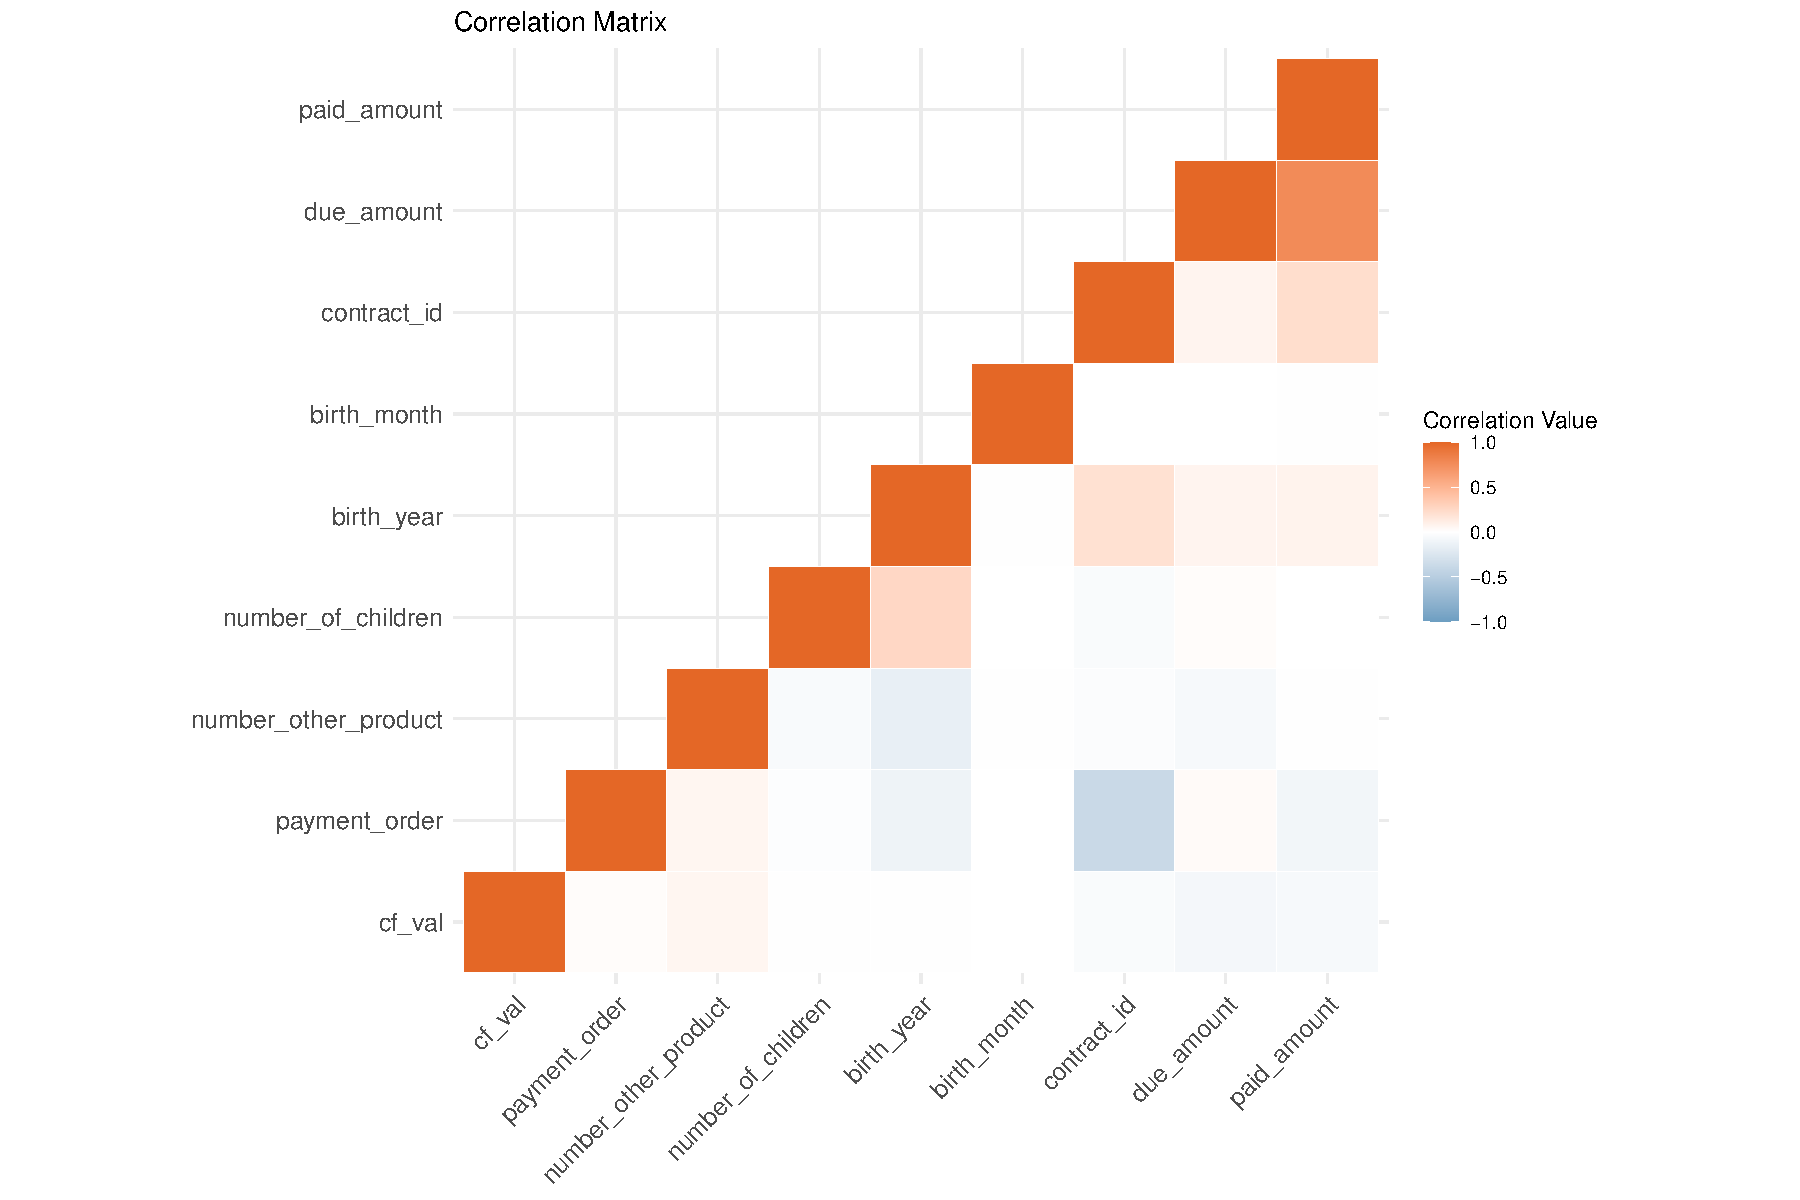
\includegraphics{Documentation_Rmarkdown_files/figure-latex/correlogram-1.pdf}
\caption{\label{fig:correlogram}\label{fig:correlogram}Correlation plot.}
\end{figure}

\begin{figure}
\centering
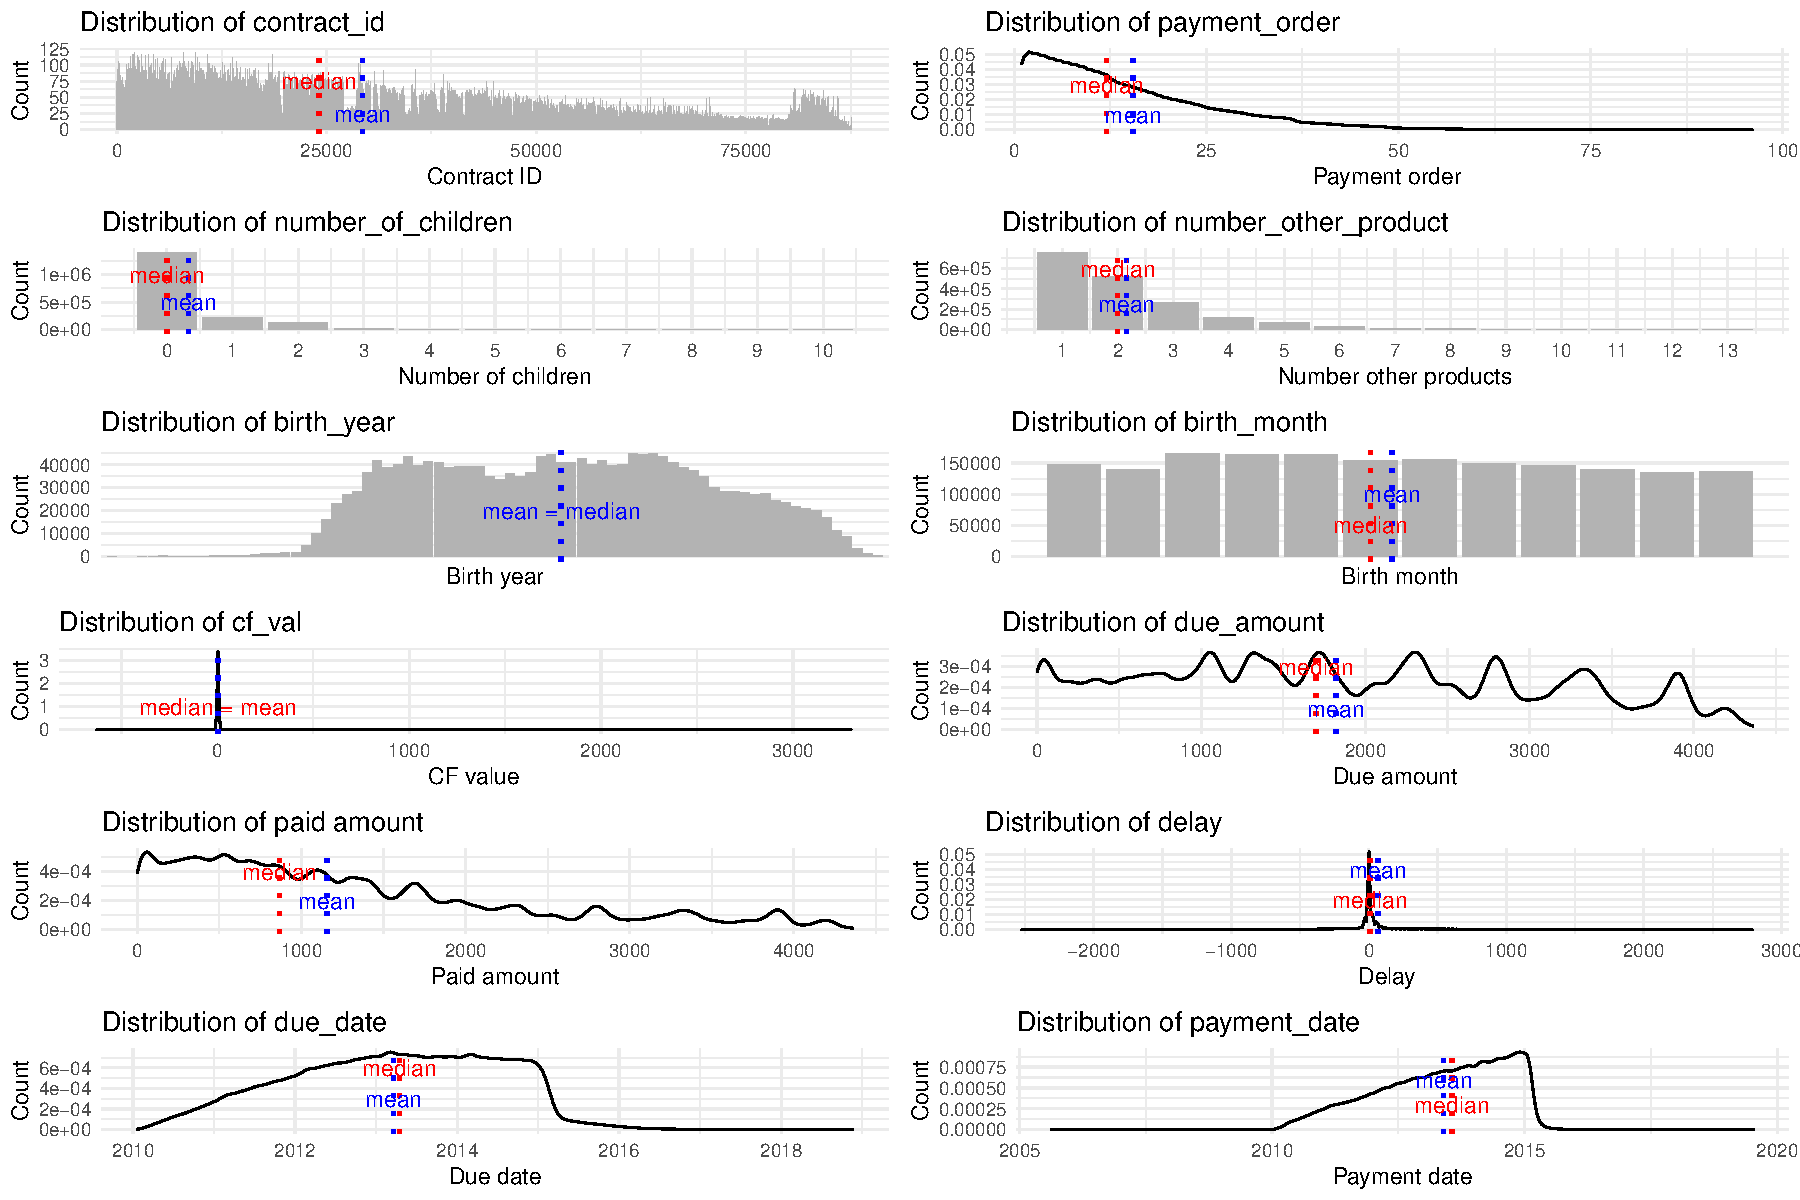
\includegraphics{Documentation_Rmarkdown_files/figure-latex/density-1.pdf}
\caption{\label{fig:density}\label{fig:density}Density plots.}
\end{figure}

\begin{figure}
\centering
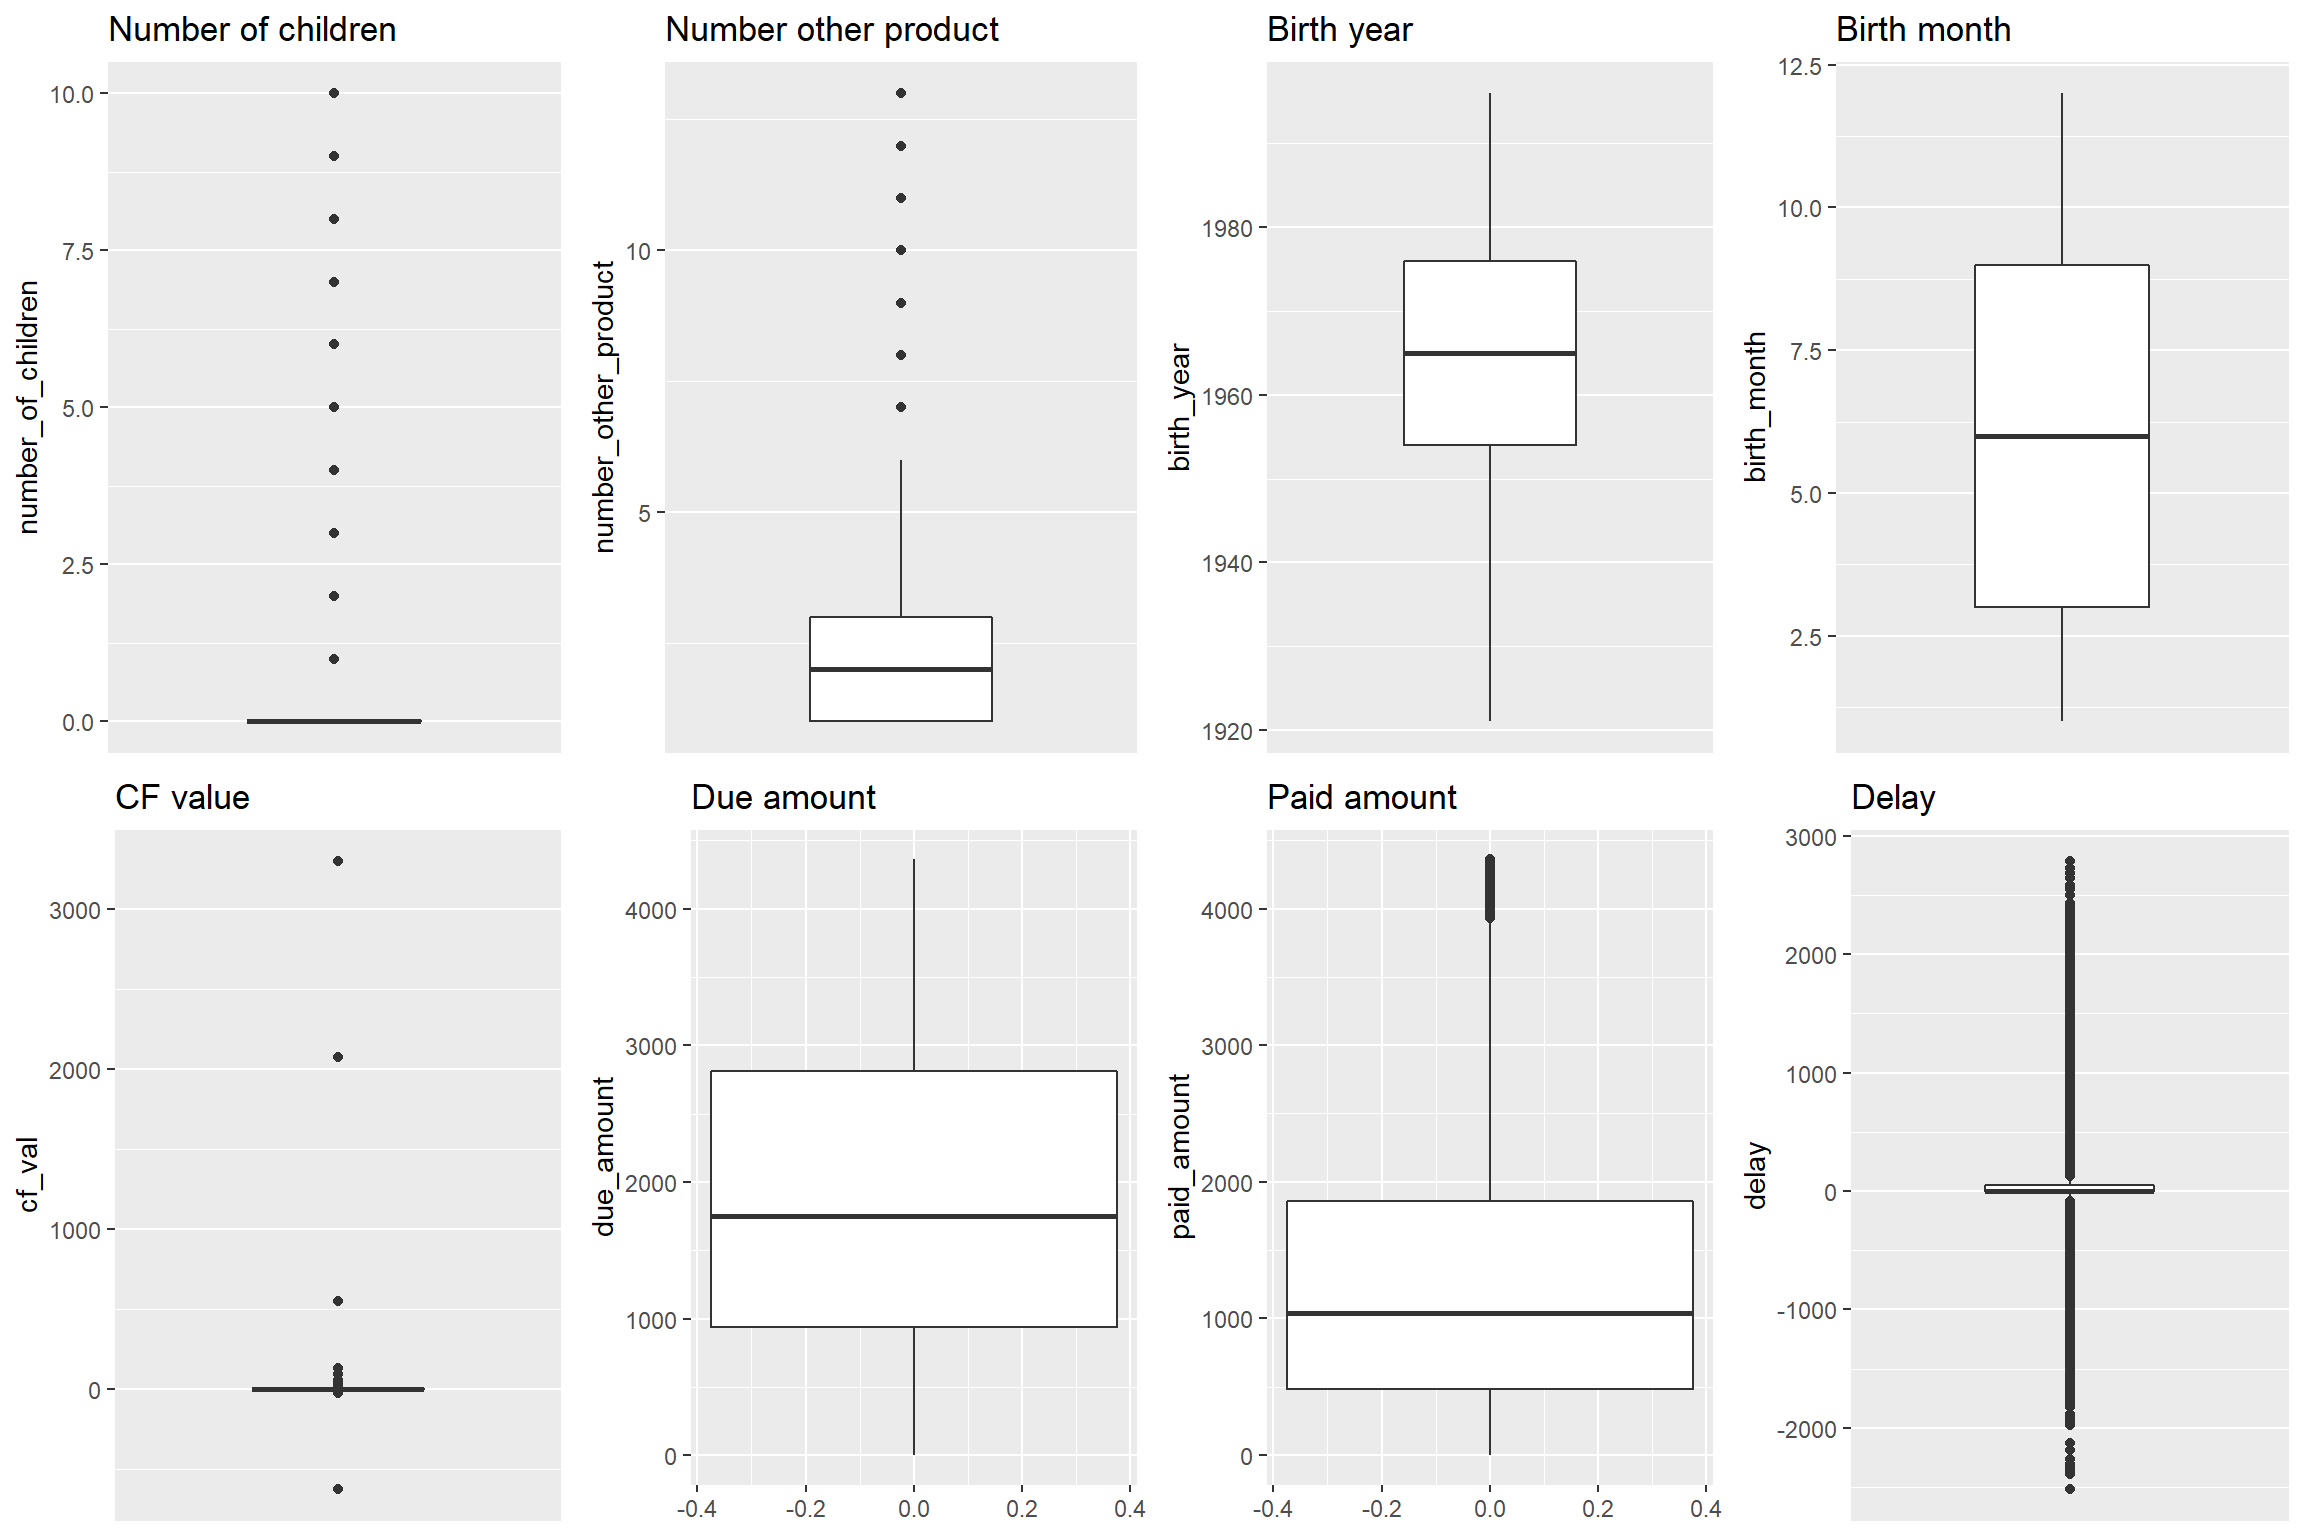
\includegraphics{Documentation_Rmarkdown_files/figure-latex/boxplots-1.pdf}
\caption{\label{fig:boxplots}\label{fig:boxplots}Boxplots for numeric attributes.}
\end{figure}

\begin{figure}
\centering
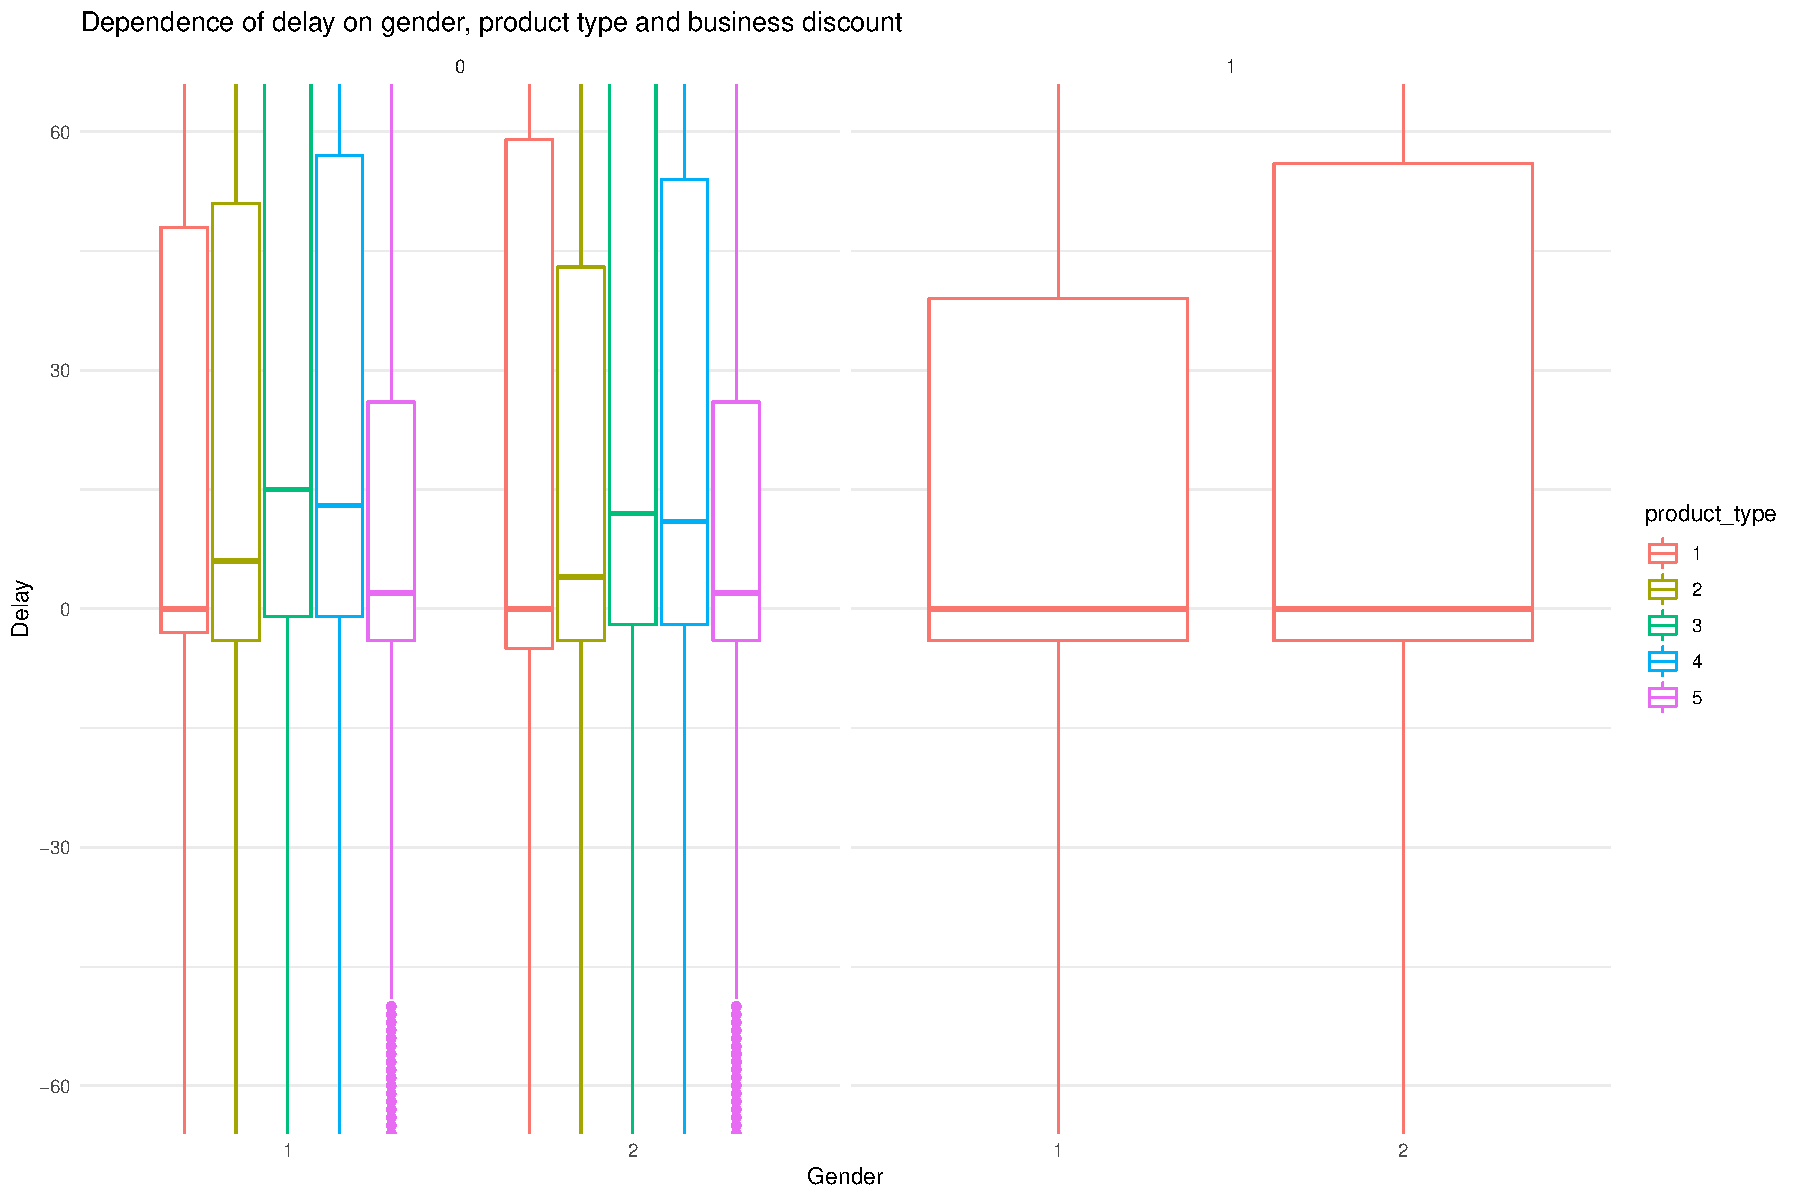
\includegraphics{Documentation_Rmarkdown_files/figure-latex/delay-gender-prod-1.pdf}
\caption{\label{fig:delay-gender-prod}\label{fig:delay-gender-prod}Dependence of delay on gender, product type and business discount.}
\end{figure}

\begin{figure}
\centering
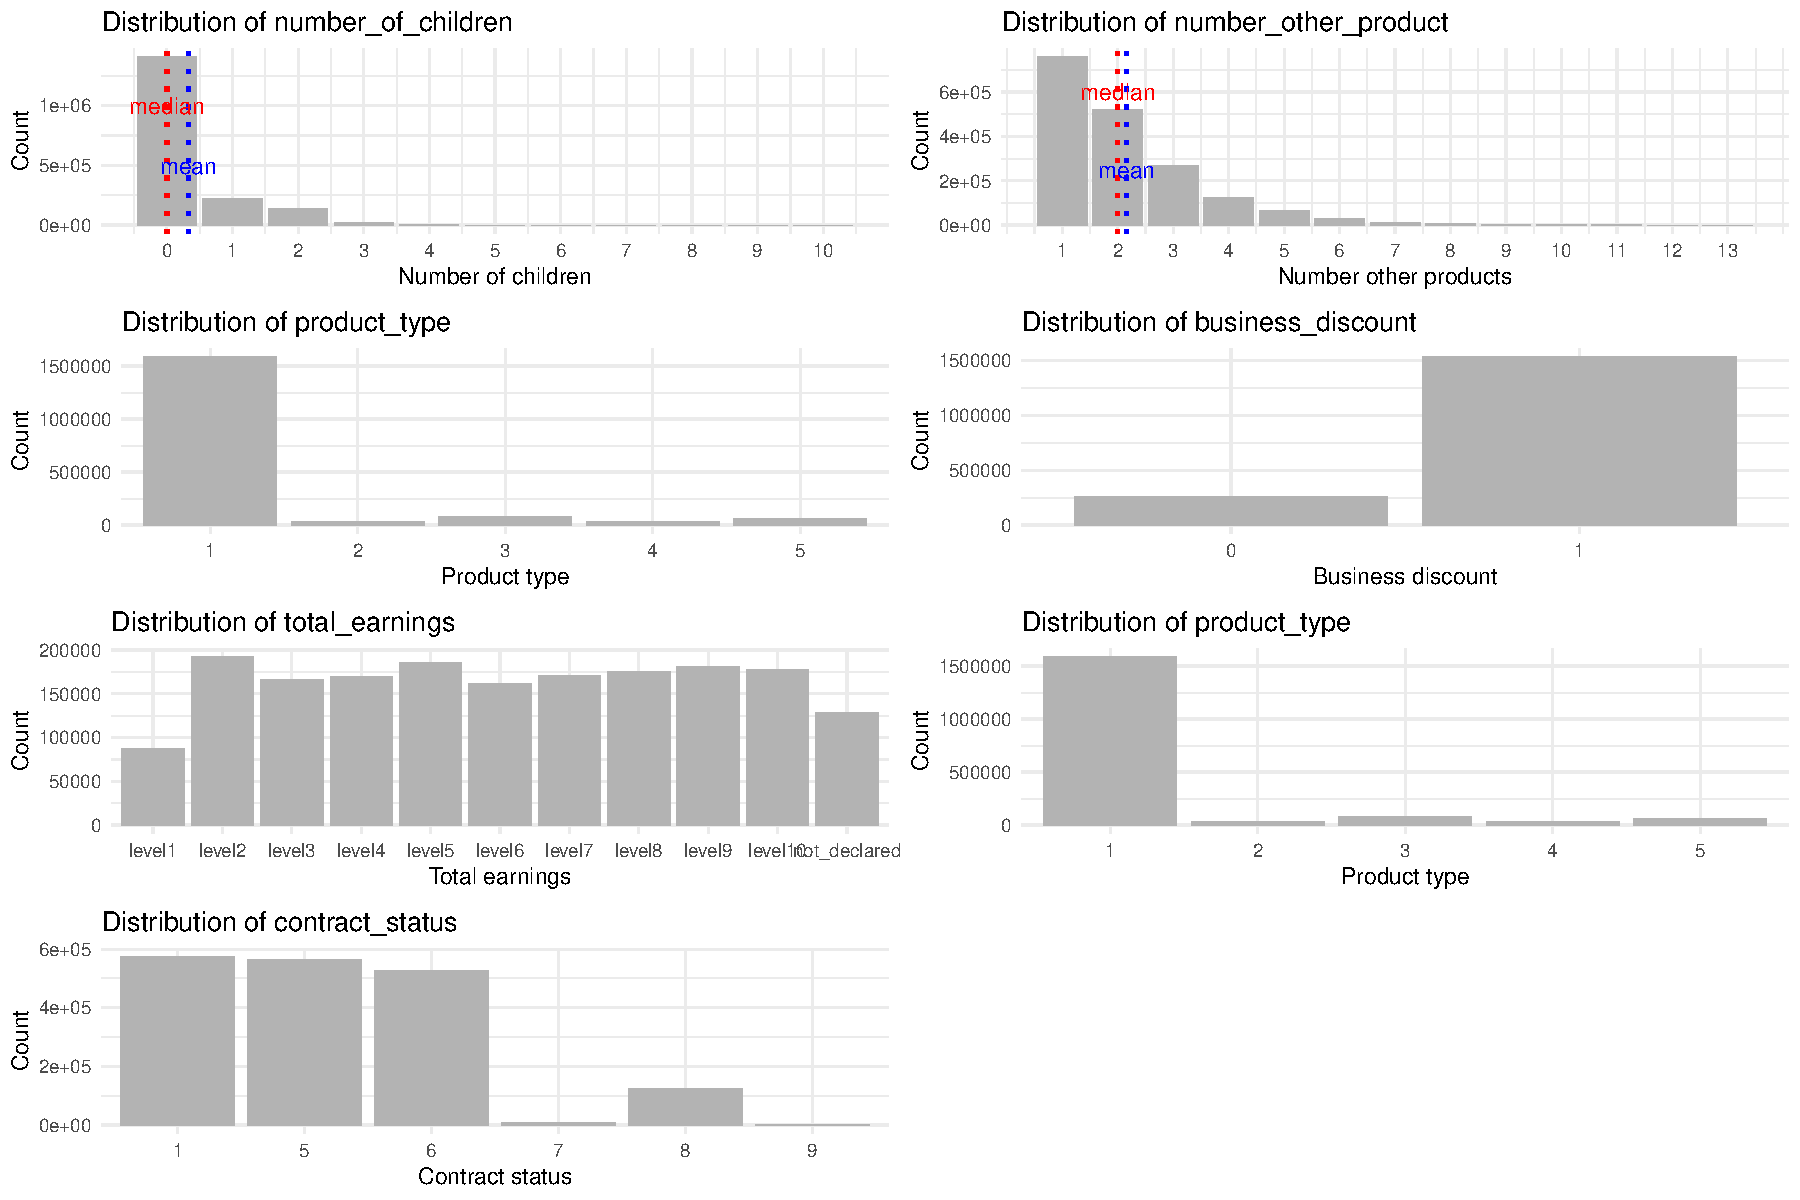
\includegraphics{Documentation_Rmarkdown_files/figure-latex/distribution-1.pdf}
\caption{\label{fig:distribution}Distribution plots.}
\end{figure}

\begin{figure}
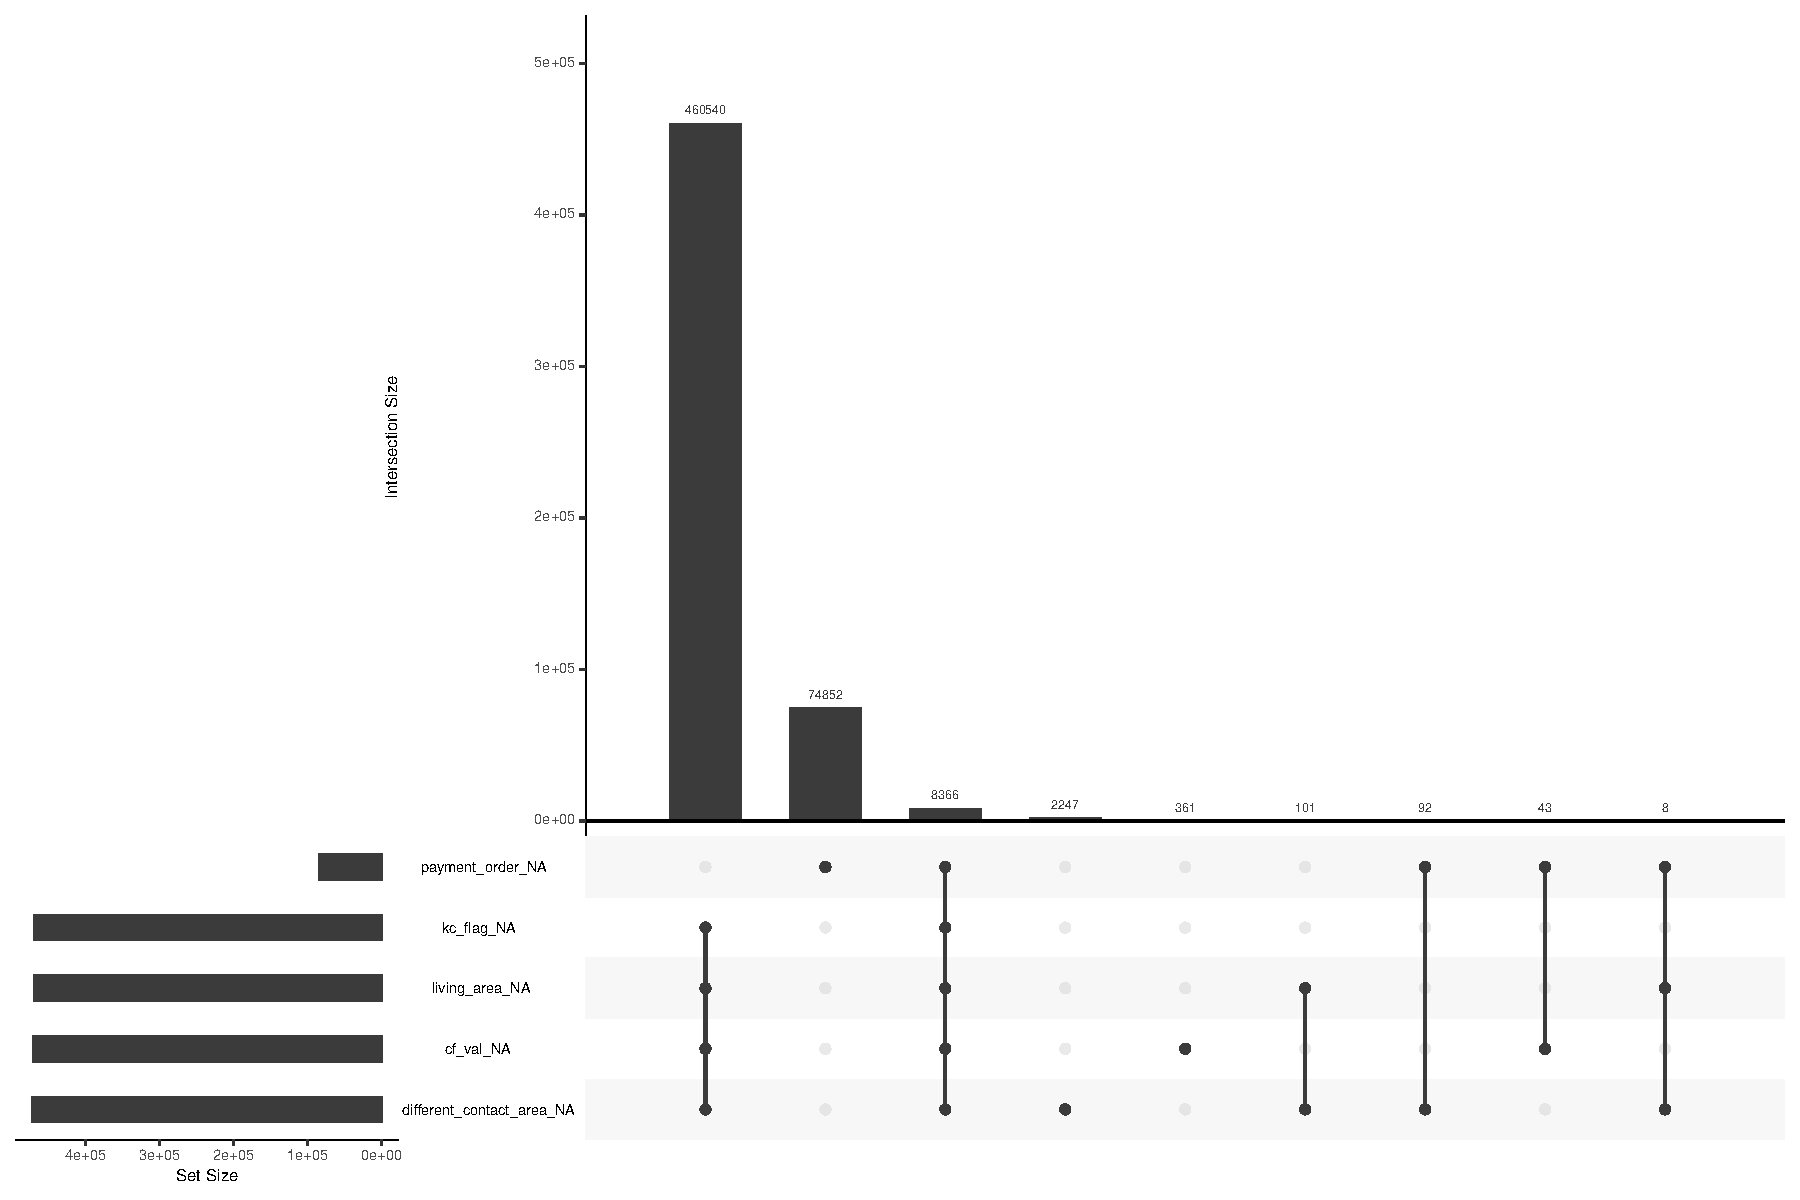
\includegraphics[width=0.9\linewidth]{Documentation_Rmarkdown_files/figure-latex/Missing-complex-1} \caption{\label{fig:Missing-complex}Distribution of missing values.}\label{fig:Missing-complex}
\end{figure}

\begin{figure}
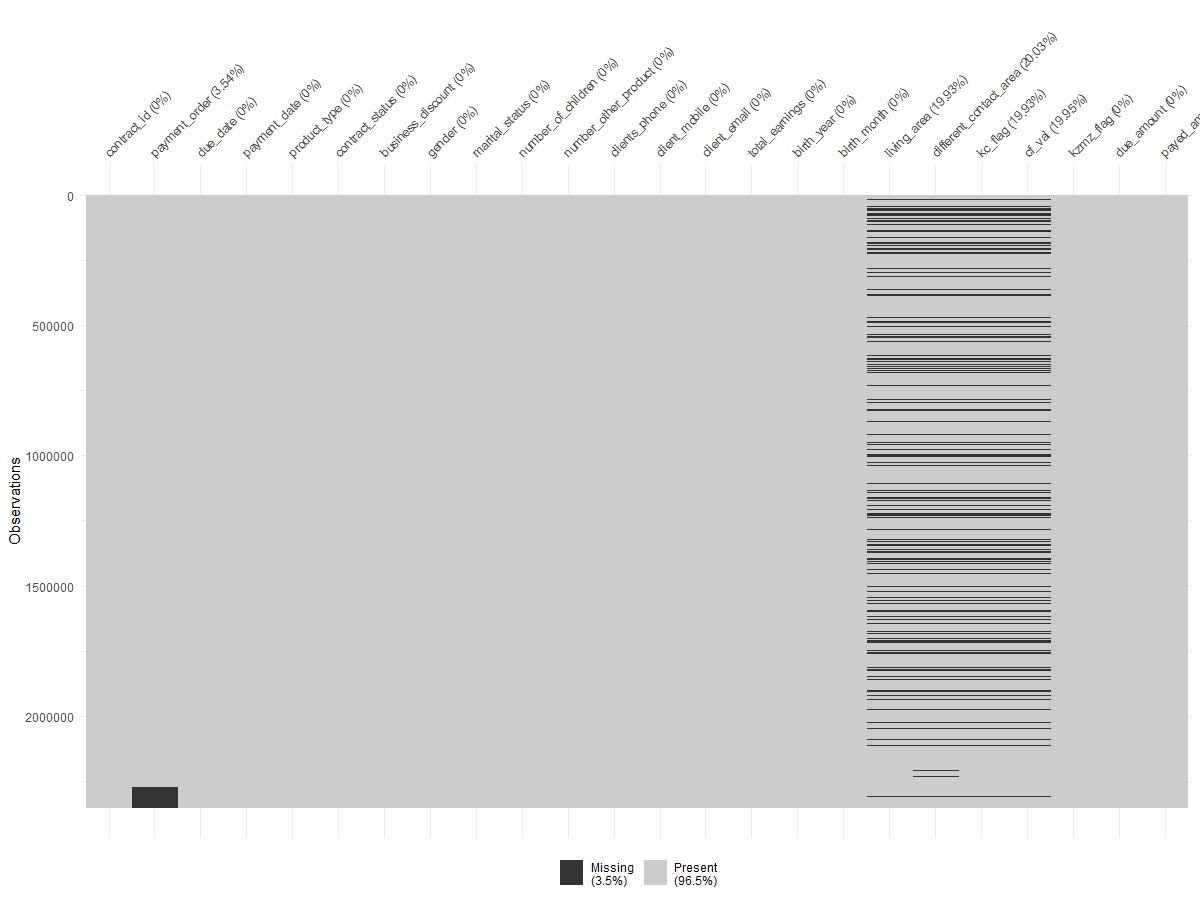
\includegraphics[width=0.9\linewidth]{missing_values_plot} \caption{\label{fig:missing-H}Distribution of missing values}\label{fig:missing-H}
\end{figure}

\begin{figure}
\centering
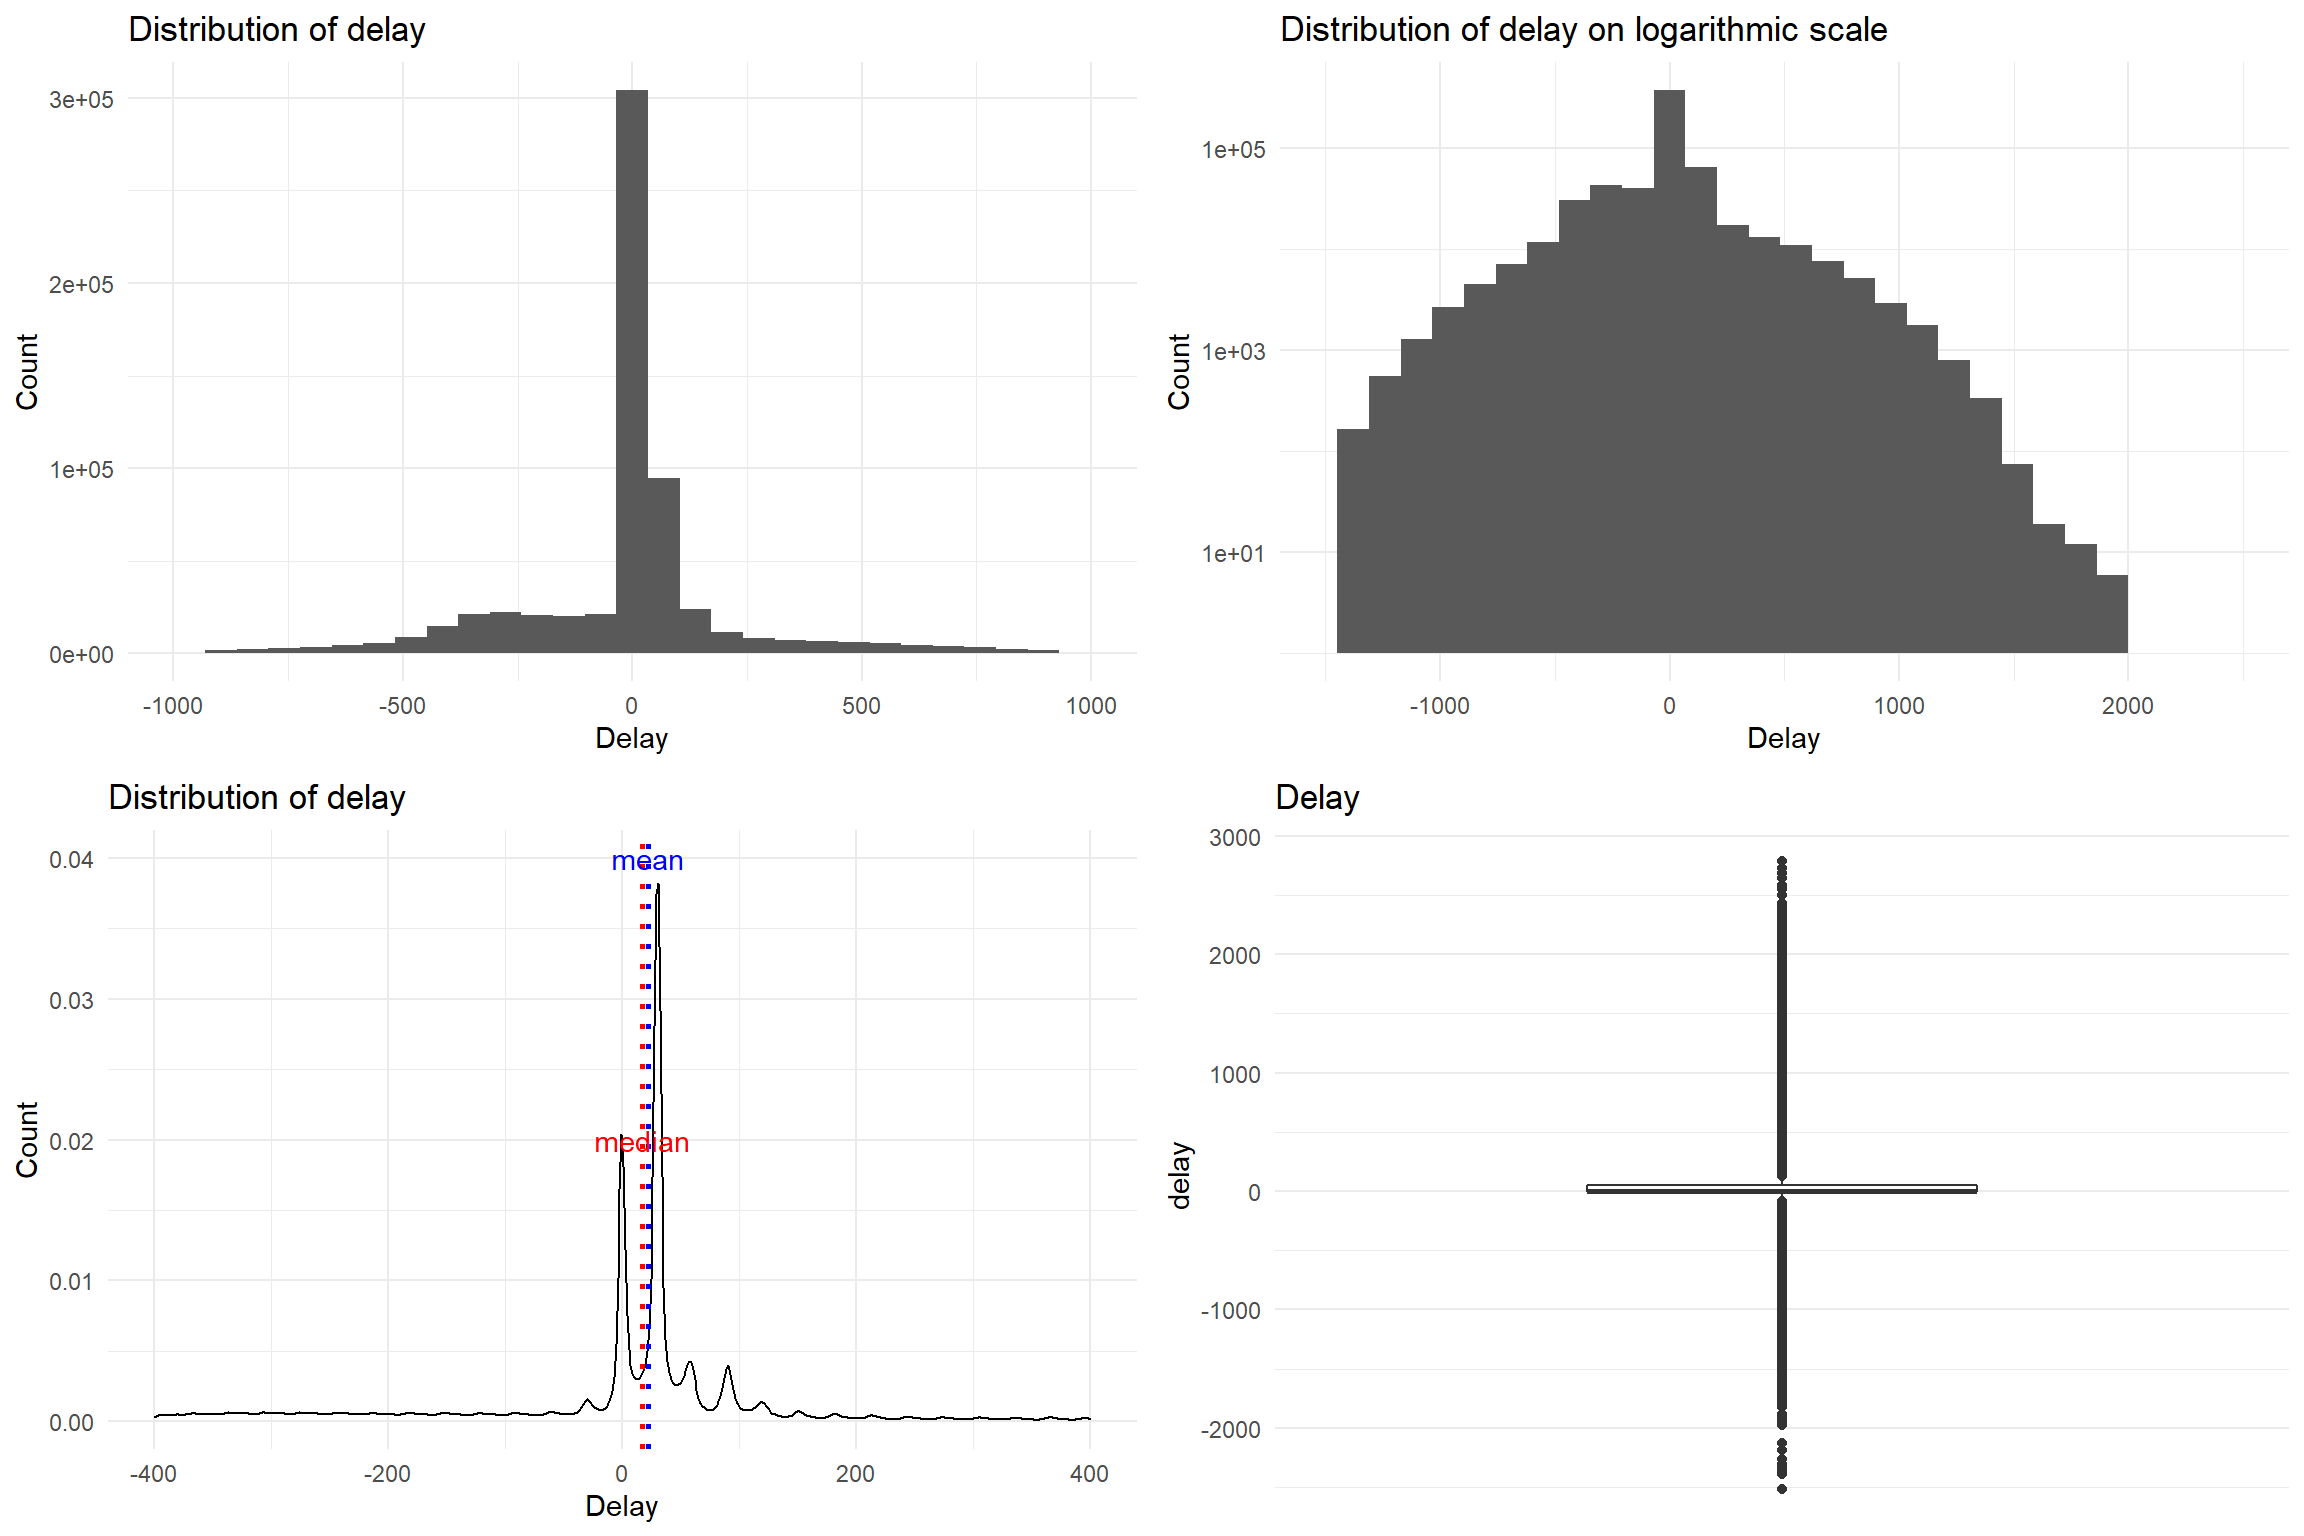
\includegraphics{Documentation_Rmarkdown_files/figure-latex/statnewdelay-1.pdf}
\caption{\label{fig:statnewdelay}\label{fig:stat-newdelay}Basic statistics of the added attribute delay.}
\end{figure}

\begin{figure}
\centering
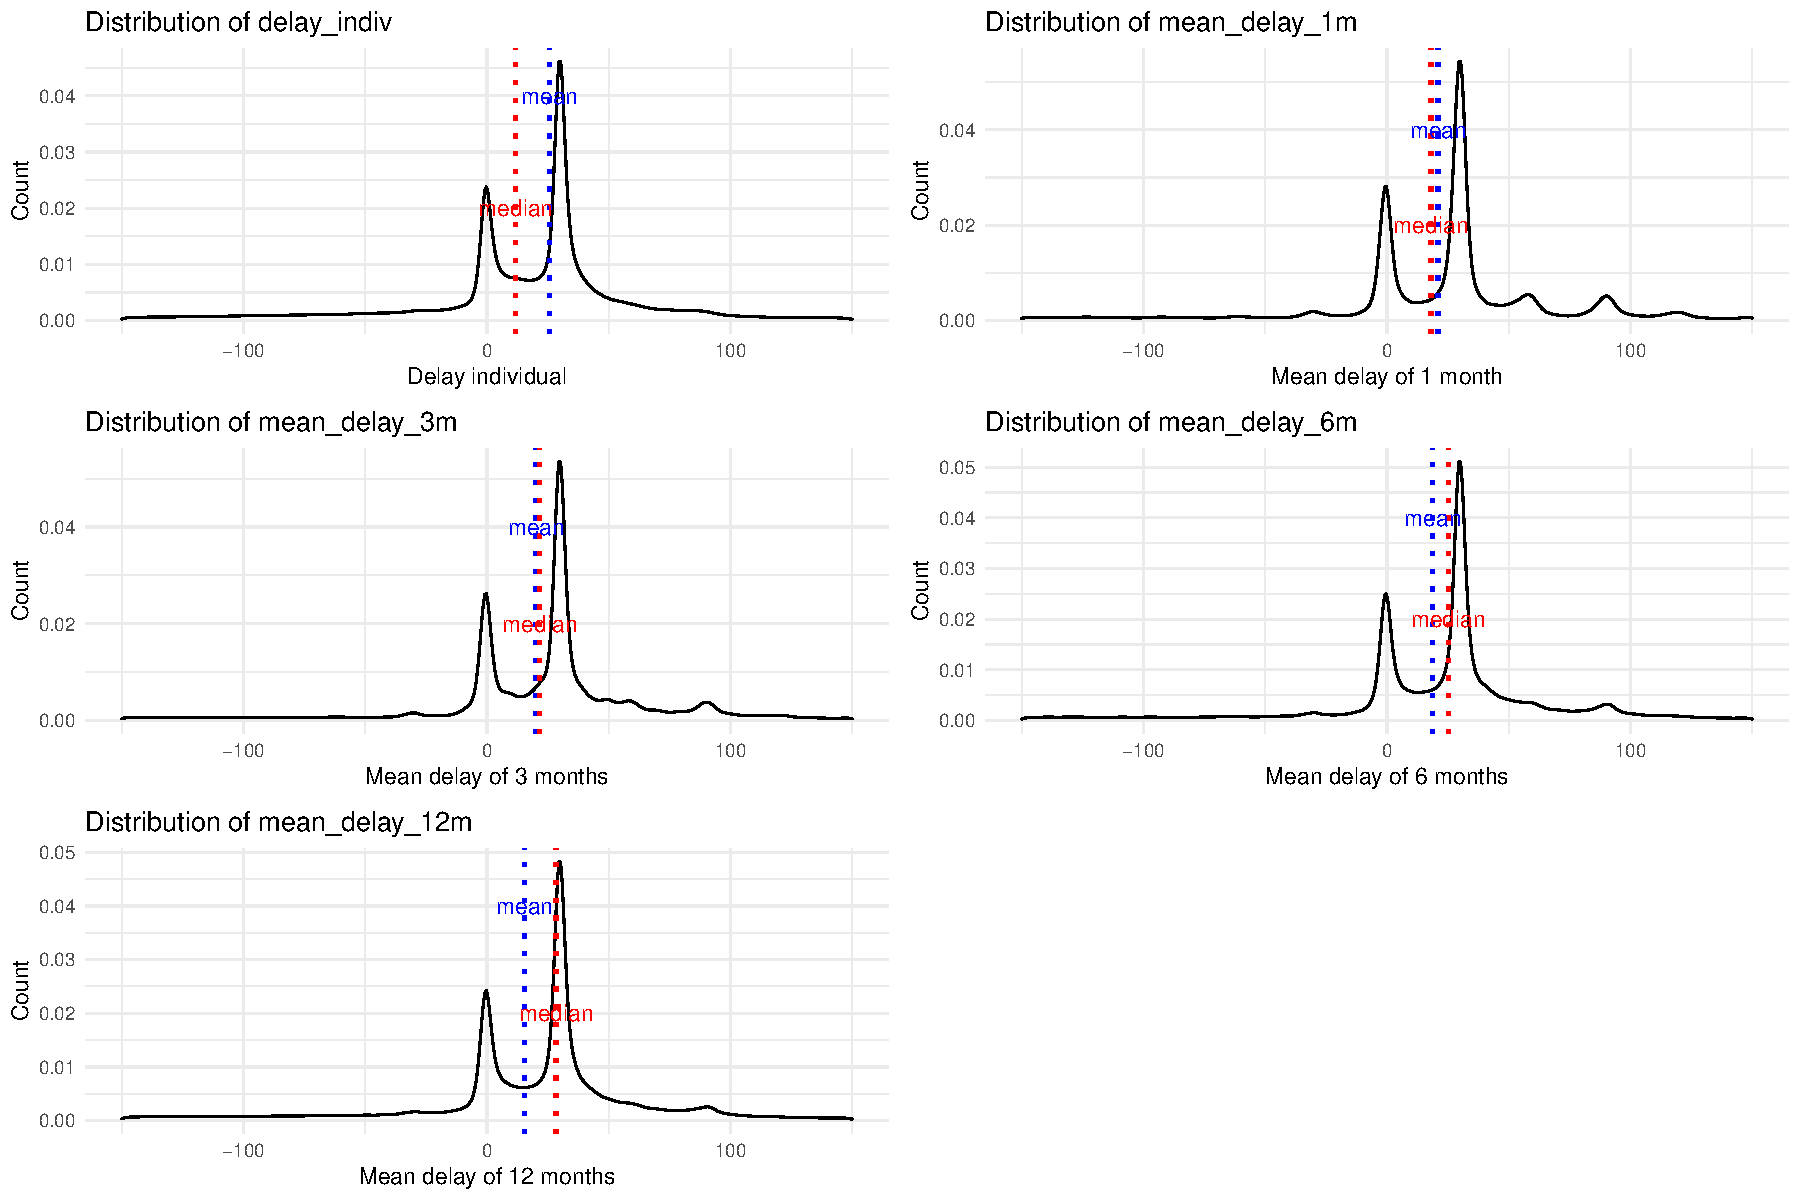
\includegraphics{Documentation_Rmarkdown_files/figure-latex/statnew-1.pdf}
\caption{\label{fig:statnew}\label{fig:stat-new}Basic statistics of the added attributes.}
\end{figure}

\begin{figure}
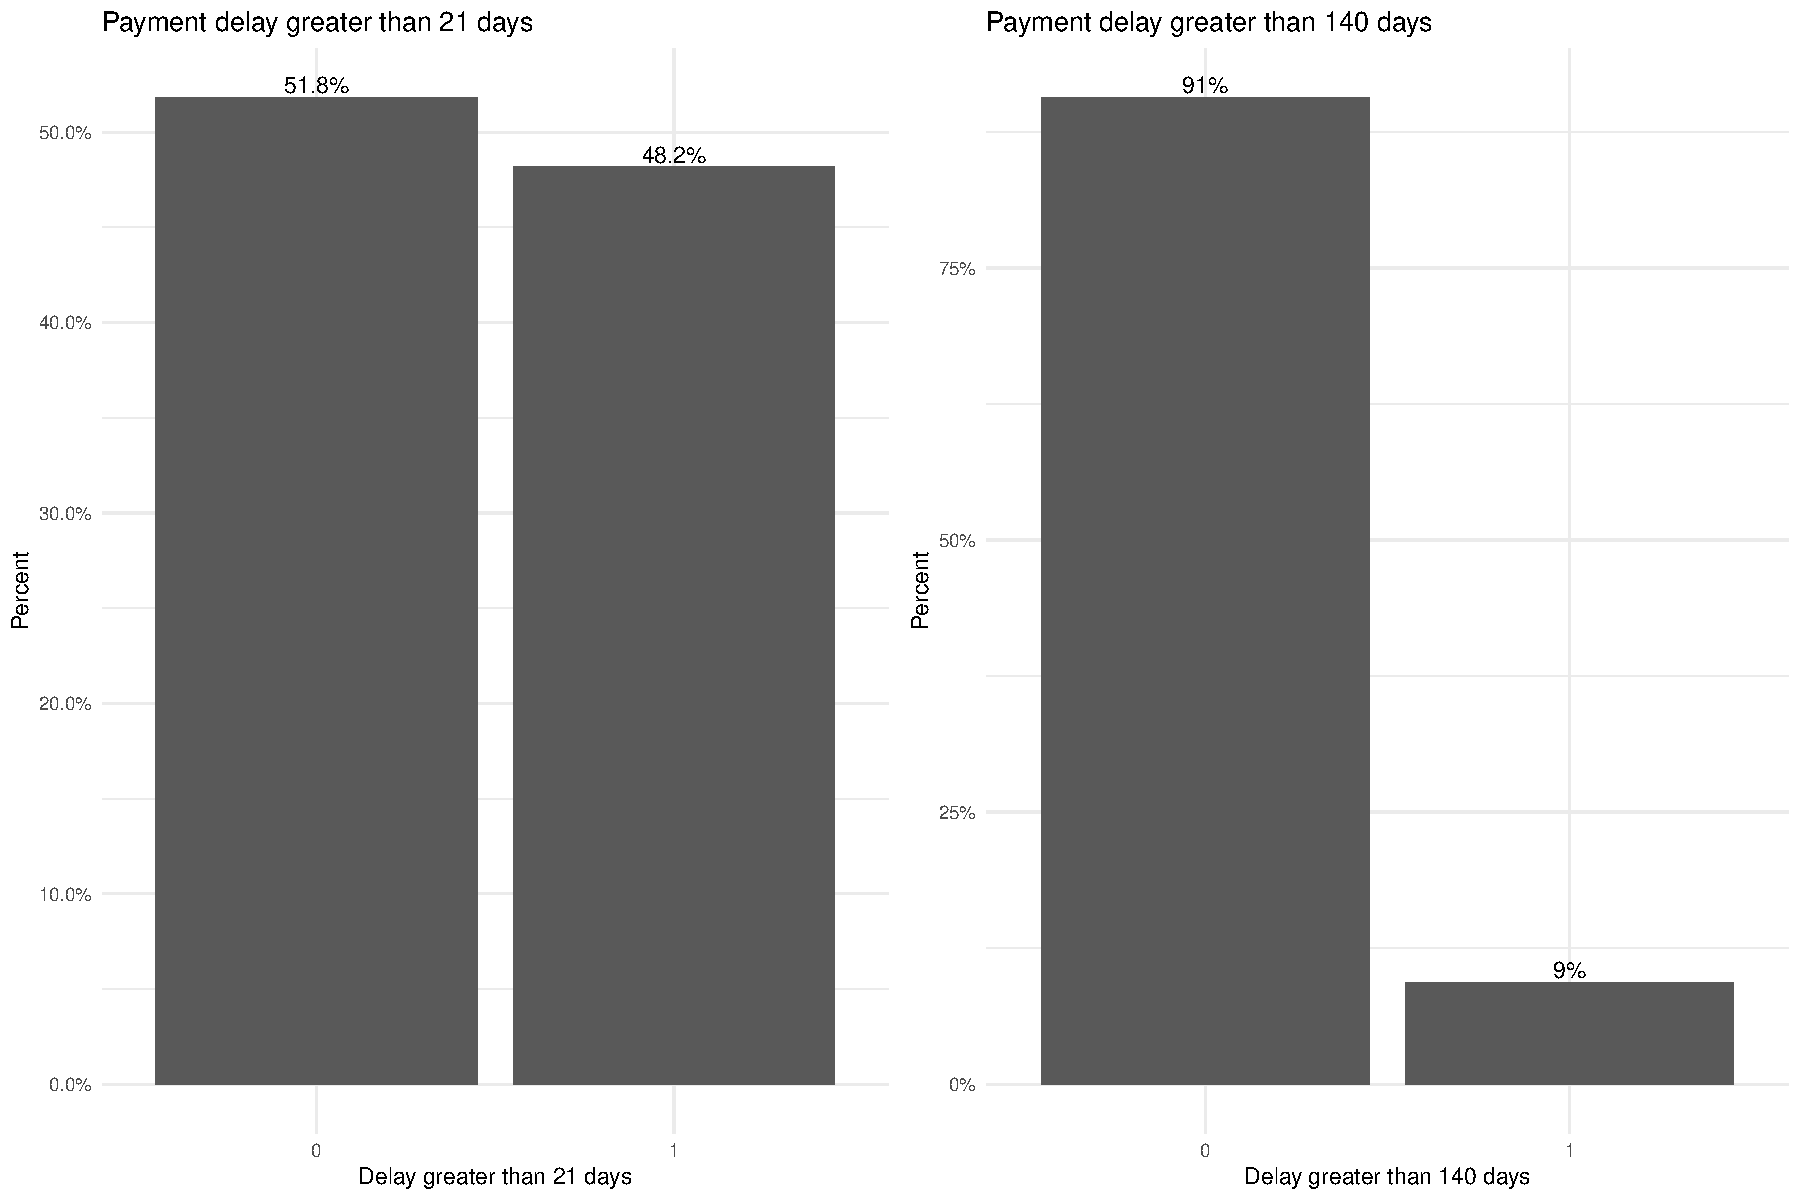
\includegraphics[height=0.4\textheight]{Documentation_Rmarkdown_files/figure-latex/helpnew-1} \caption{\label{fig:help_new} Statistics of the factor added attributes.}\label{fig:helpnew}
\end{figure}

\begin{figure}
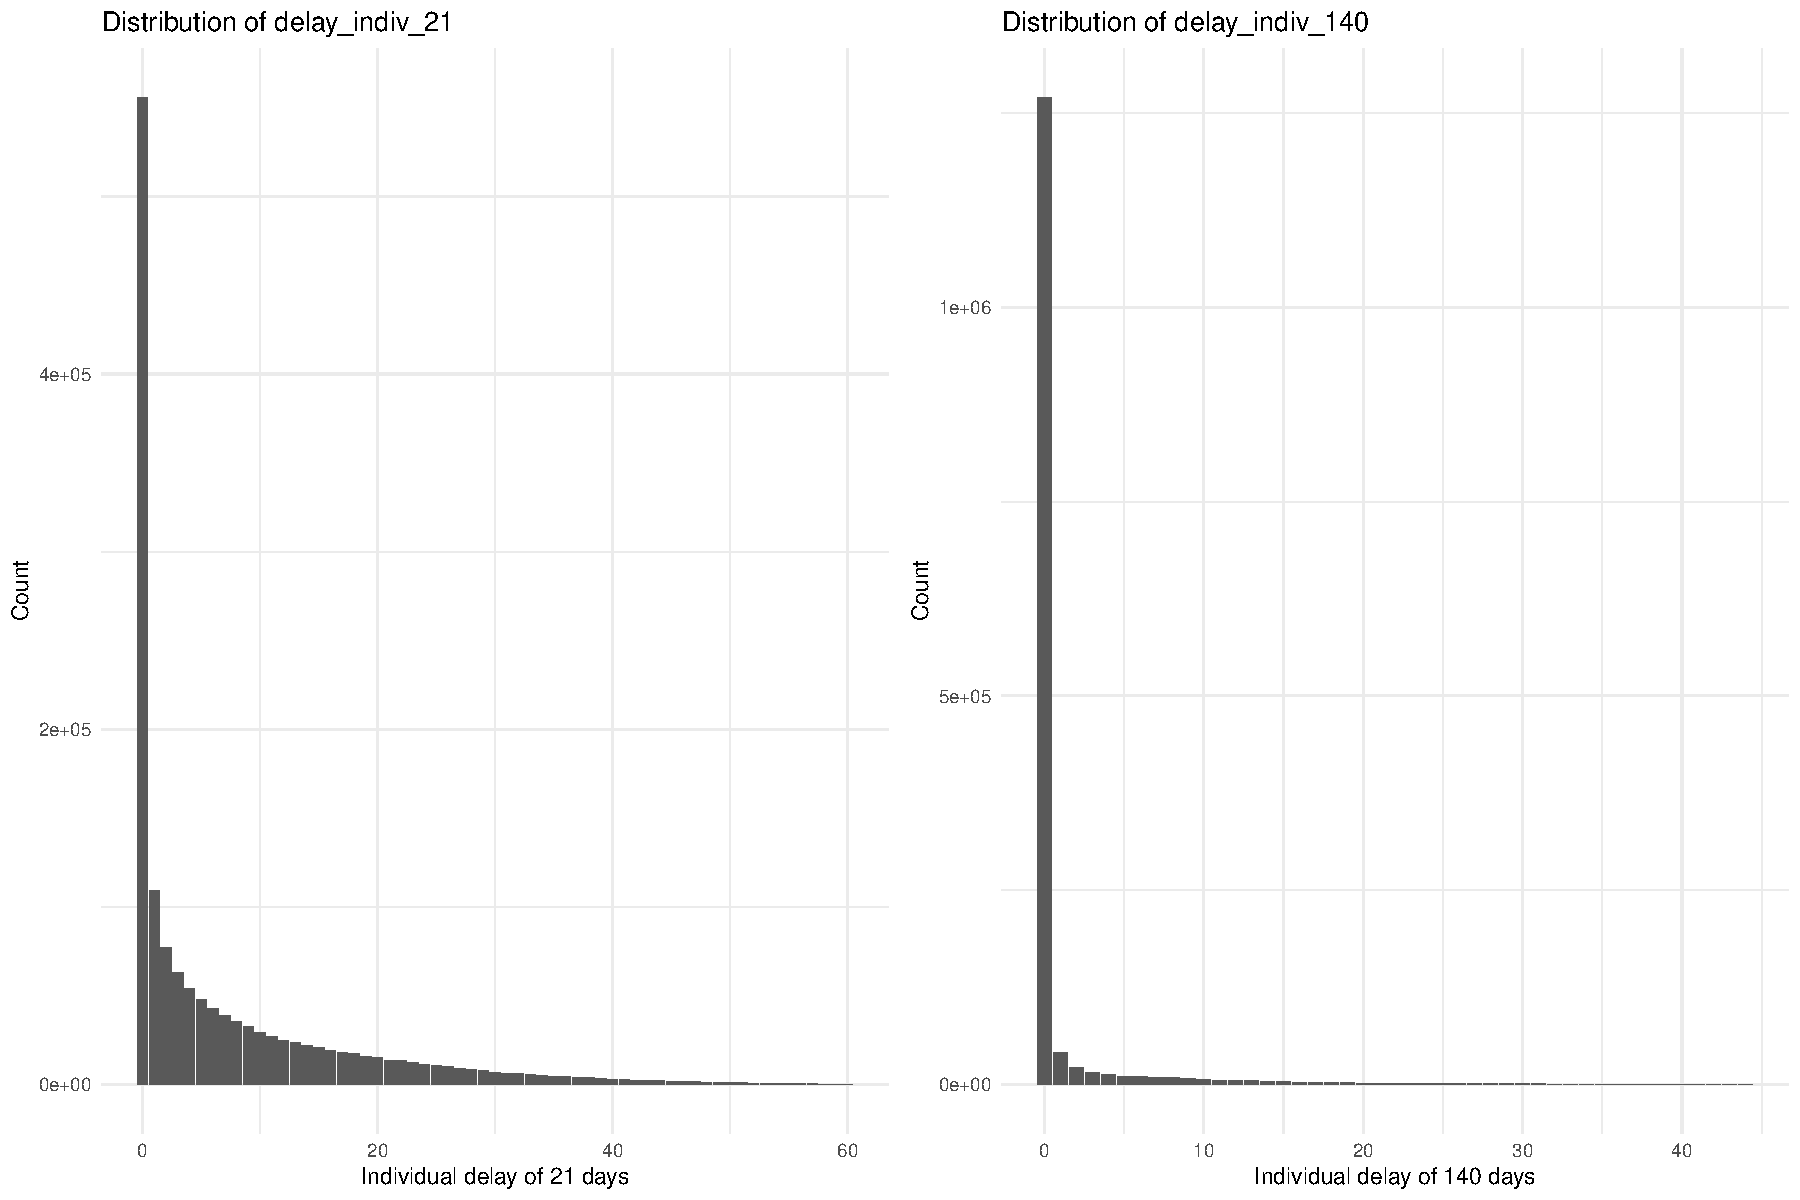
\includegraphics[height=0.4\textheight]{Documentation_Rmarkdown_files/figure-latex/statIndiv-1} \caption{\label{fig:stat-new}Basic statistics of the added attributes.}\label{fig:statIndiv}
\end{figure}

\begin{figure}
\centering
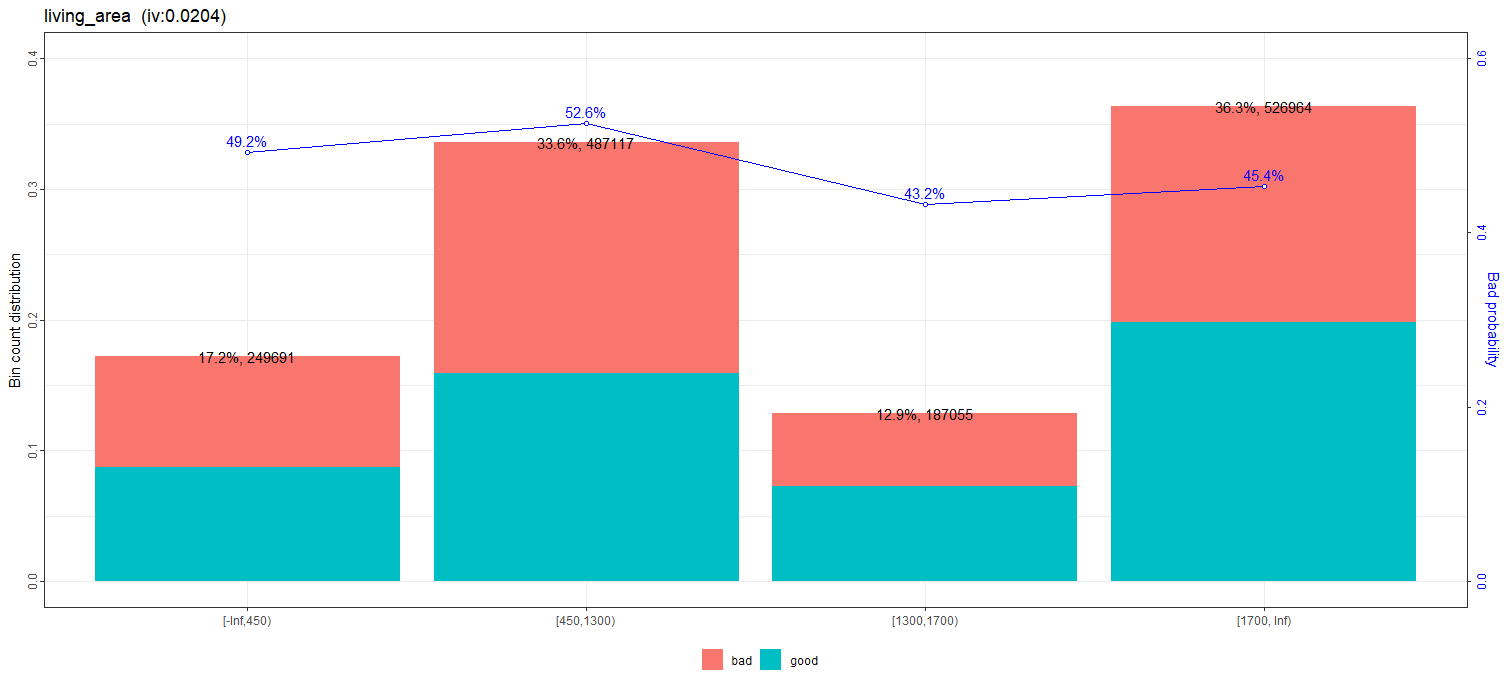
\includegraphics{.//WOE21.png}
\caption{\label{fig:woe21} Binning for living\_area (21+ delay)}
\end{figure}

\begin{figure}
\centering
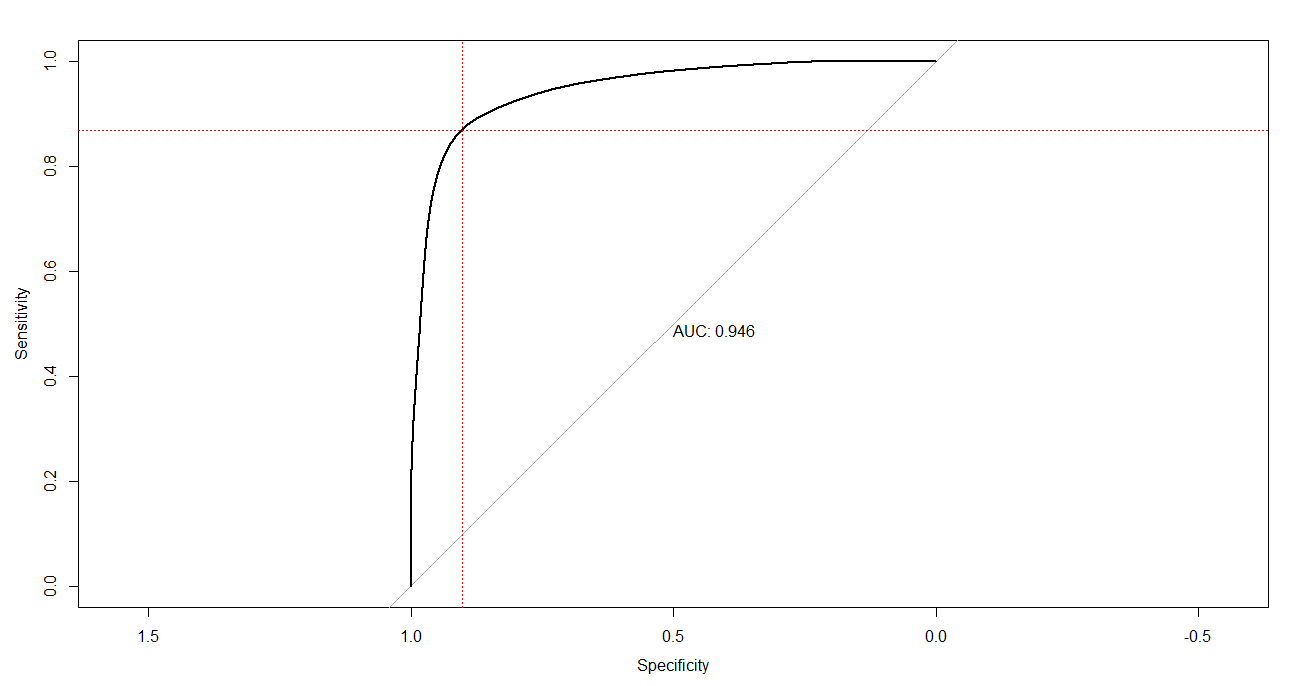
\includegraphics{.//AUC21.png}
\caption{\label{fig:auc21} ROC curve and AUC (21+ delay)}
\end{figure}

\begin{figure}
\centering
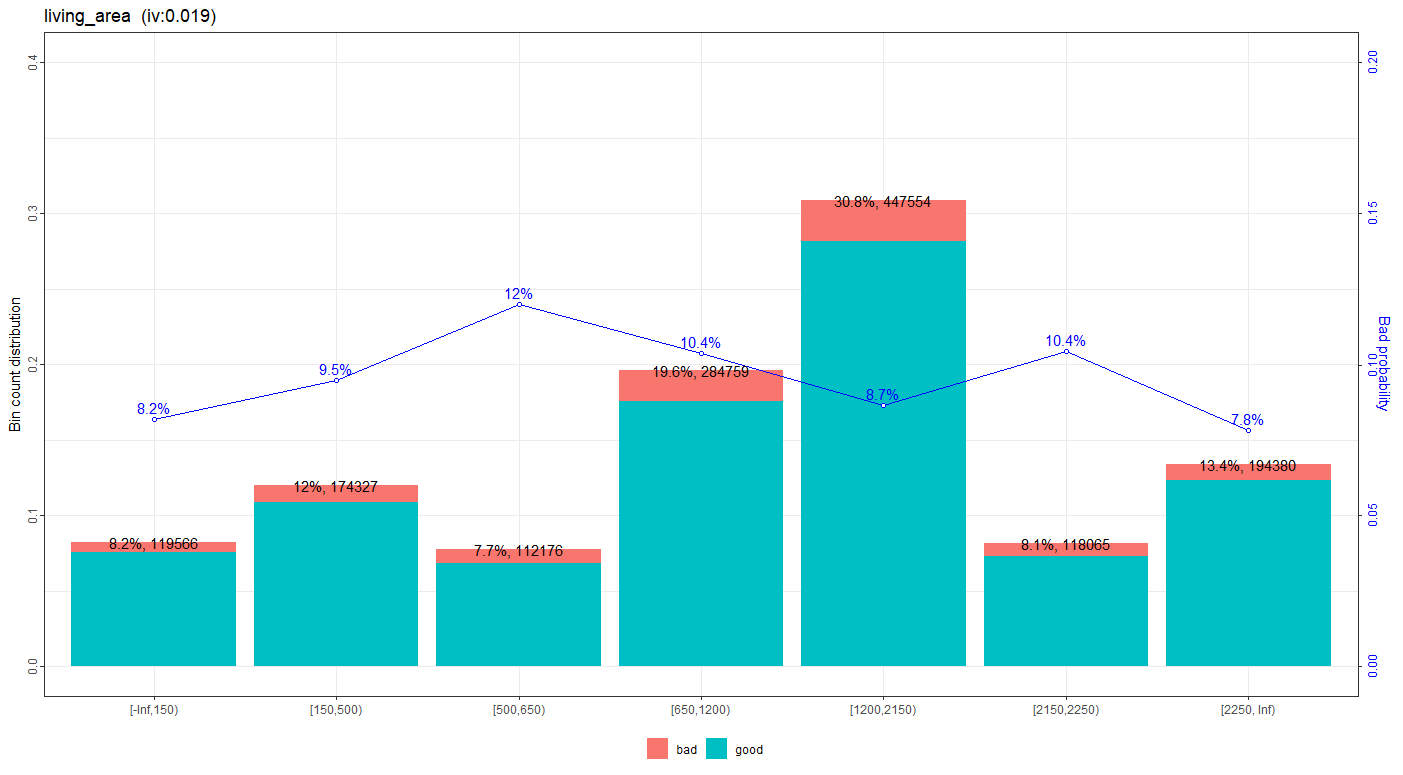
\includegraphics{.//WOE140.png}
\caption{\label{fig:woe140} Binning for living\_area (140+ delay)}
\end{figure}

\begin{figure}
\centering
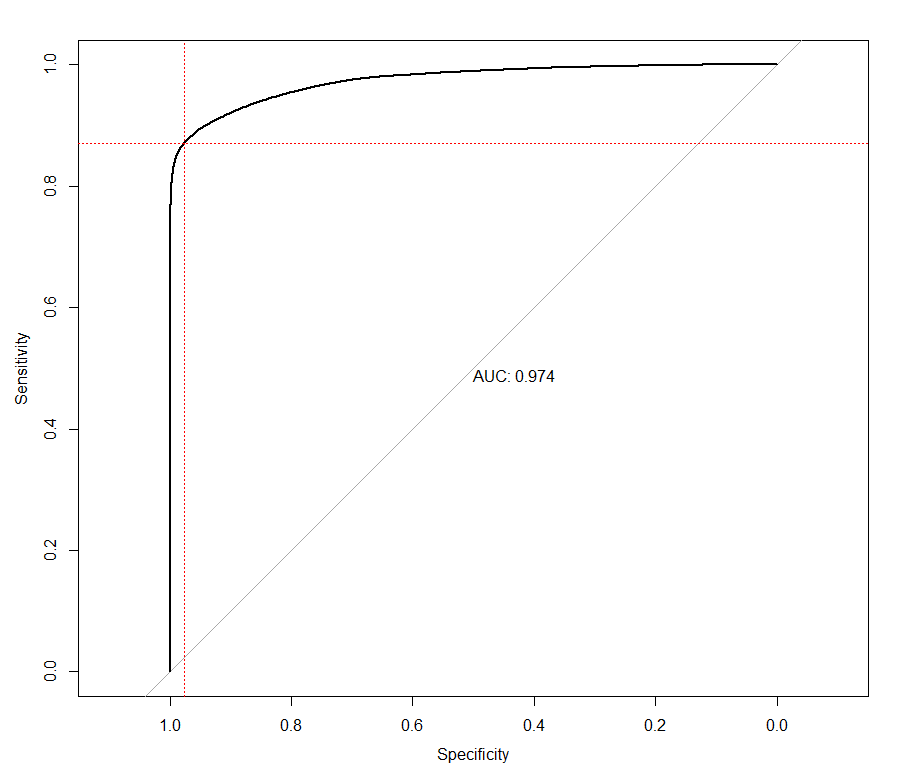
\includegraphics{.//AUC140.png}
\caption{\label{fig:auc140} ROC curve and AUC (140+ delay)}
\end{figure}

\begin{figure}
\centering
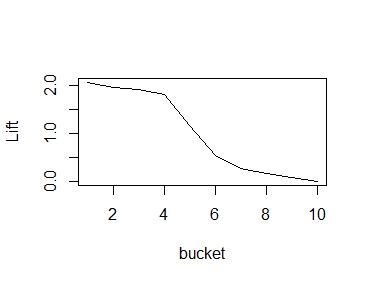
\includegraphics{.//lift21.png}
\caption{\label{fig:lift21} Lift curve (21+ delay)}
\end{figure}

\begin{figure}
\centering
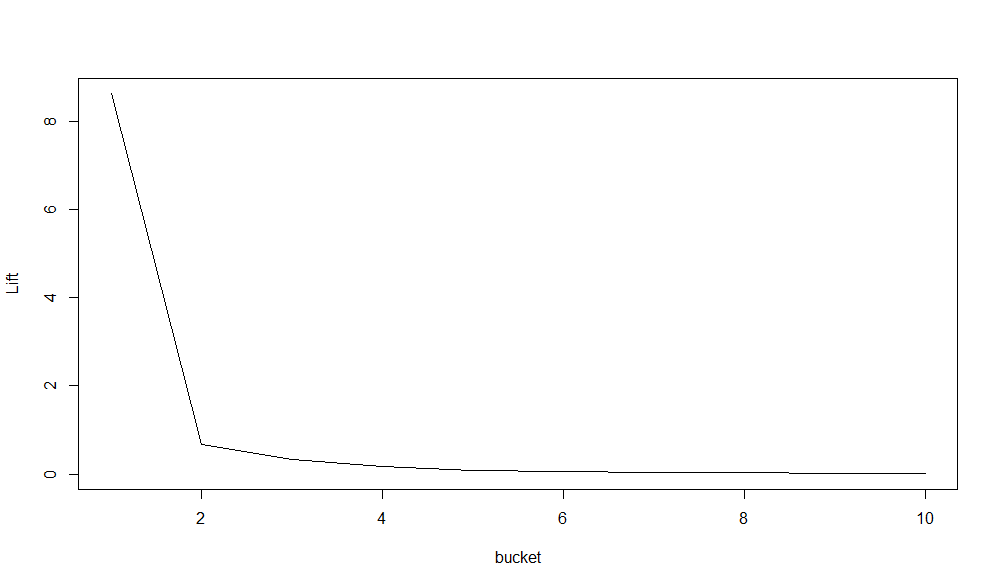
\includegraphics{.//lift140.png}
\caption{\label{fig:lift140} Lift curve (140+ delay)}
\end{figure}

\begin{figure}
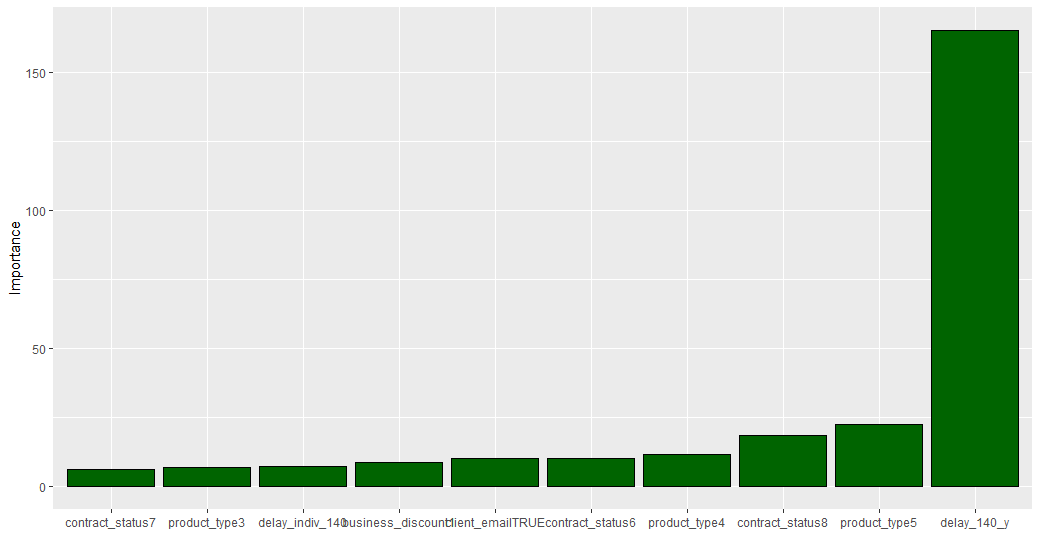
\includegraphics[width=0.9\linewidth]{delay_varImp} \caption{\label{fig:varIm}Variable importance for glmnet cv}\label{fig:varIm}
\end{figure}

\begin{figure}
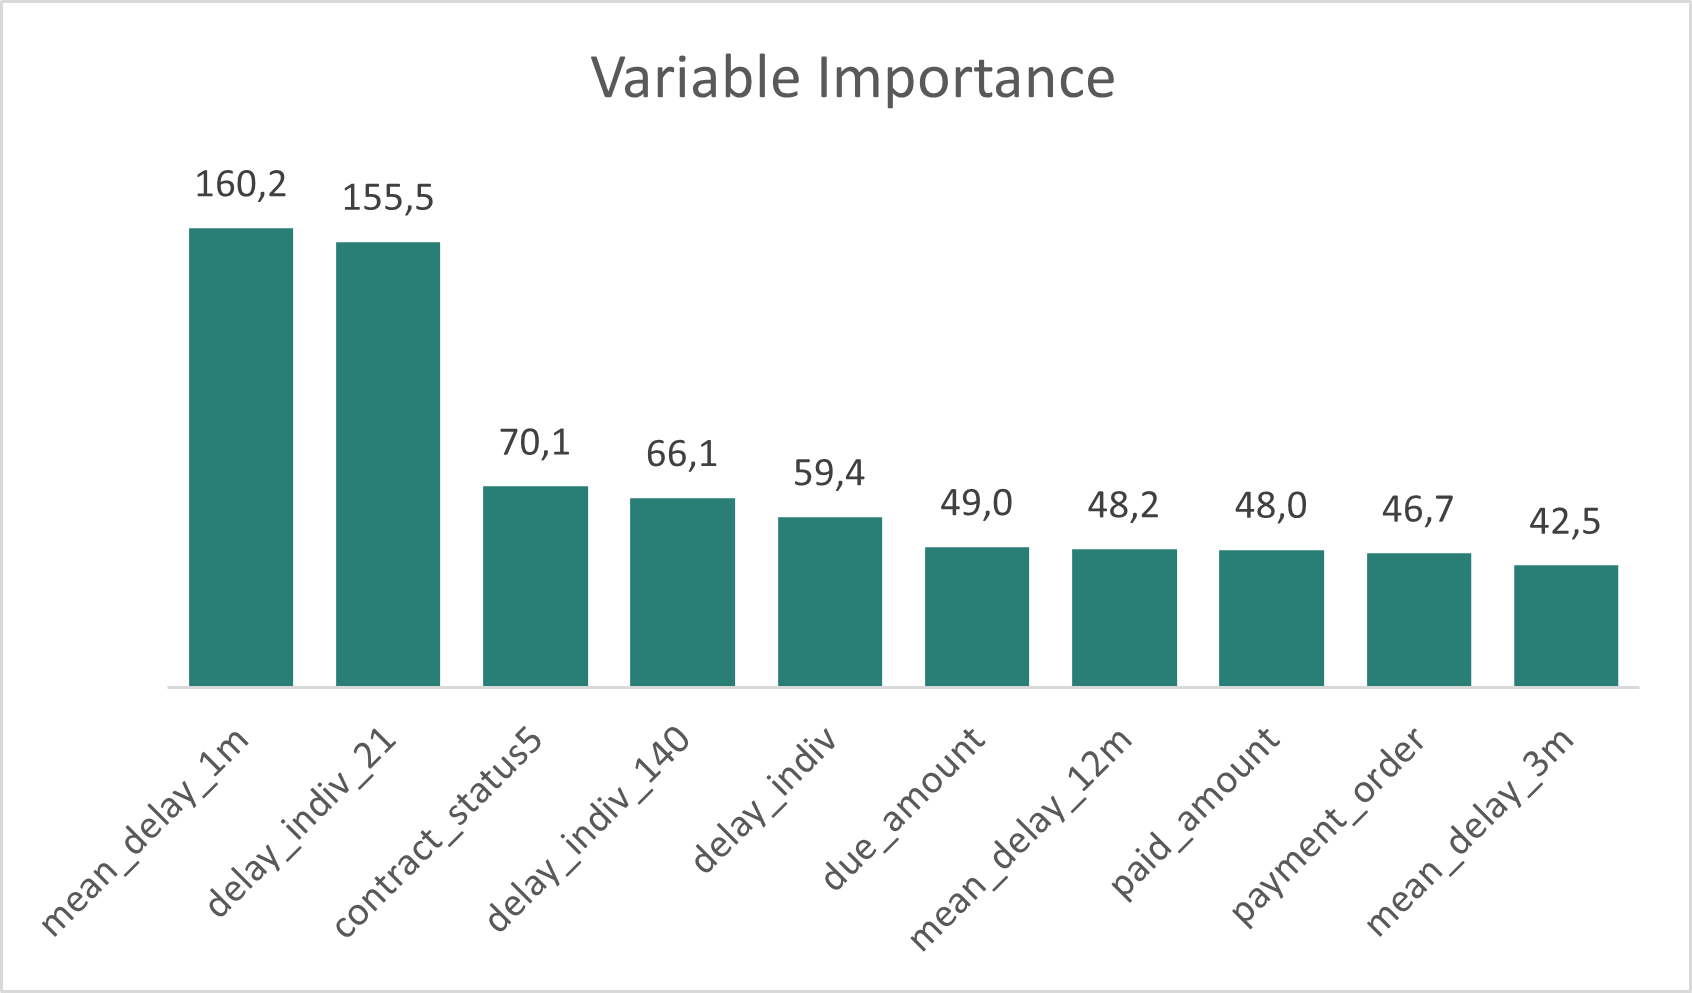
\includegraphics[width=0.9\linewidth]{varimp21} \caption{\label{fig:varIm21}Variable importance  (delay 21+)}\label{fig:varIm21}
\end{figure}

\begin{figure}
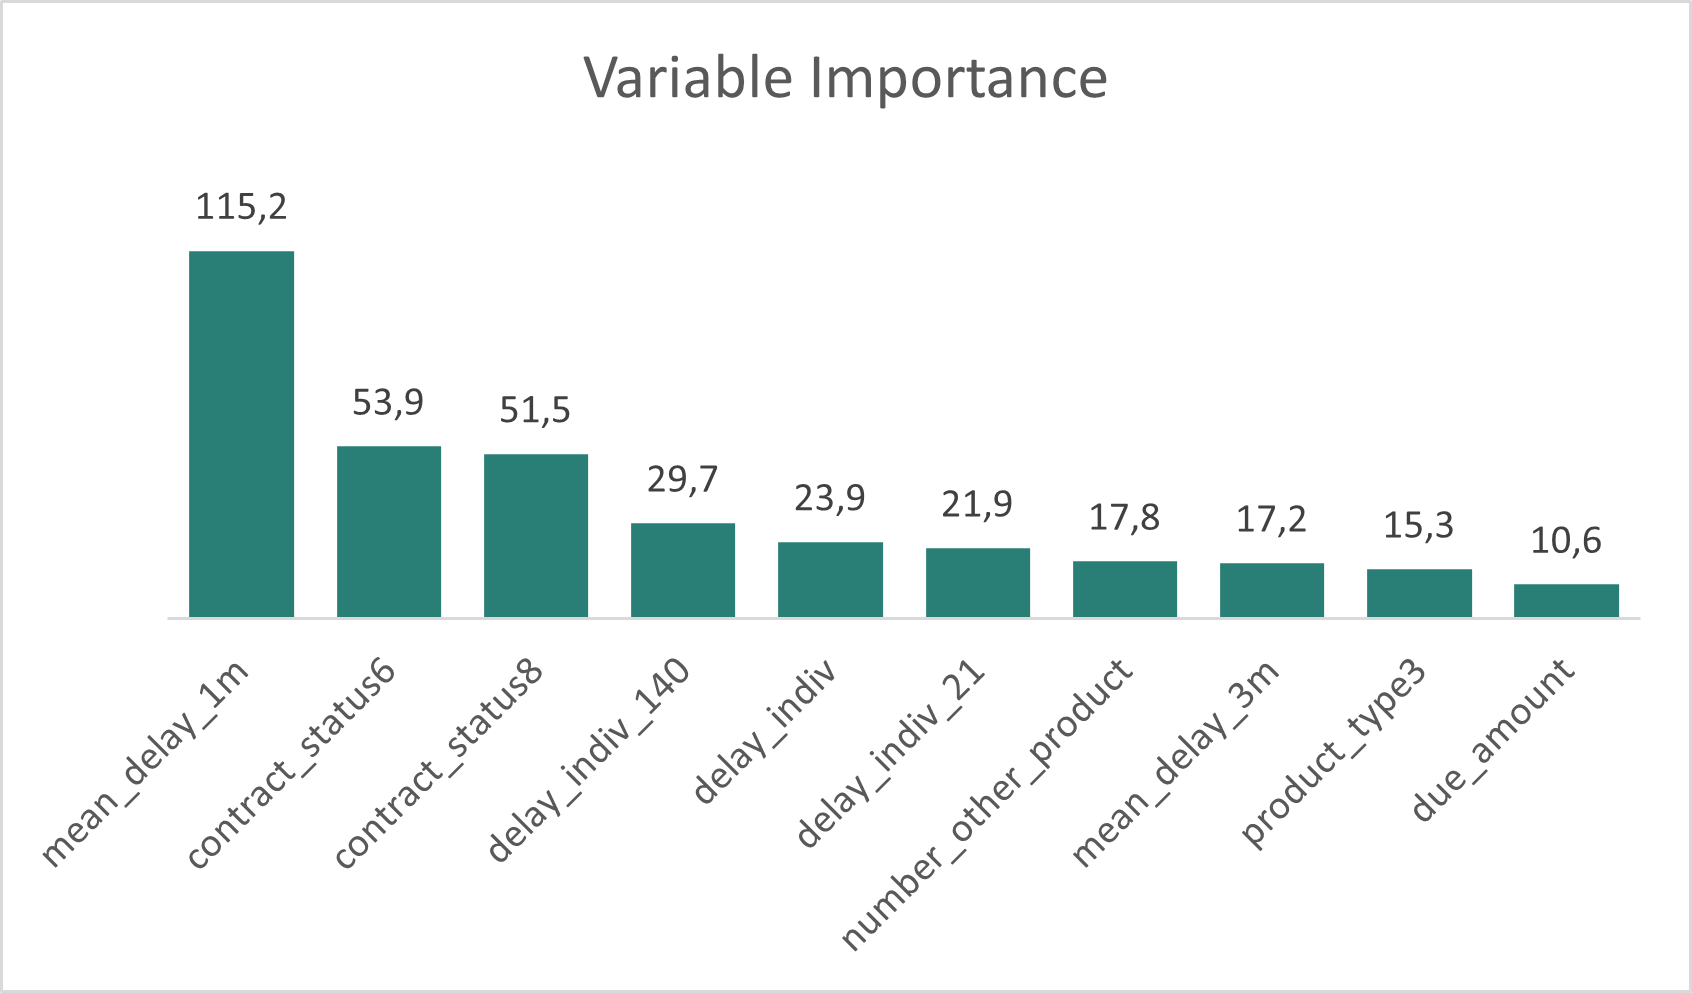
\includegraphics[width=0.9\linewidth]{varimp140} \caption{\label{fig:varIm21}Variable importance (delay 140+)}\label{fig:varIm140}
\end{figure}

\hypertarget{tables}{%
\section{Tables}\label{tables}}

\begin{table}

\caption{\label{tab:Missing-stat}Statistics of missing values.}
\centering
\begin{tabular}[t]{l|r|r}
\hline
variable & n\_miss & pct\_miss\\
\hline
different\_contact\_area & 471354 & 20.0319420\\
\hline
cf\_val & 469310 & 19.9450747\\
\hline
living\_area & 469015 & 19.9325375\\
\hline
kc\_flag & 468906 & 19.9279052\\
\hline
payment\_order & 83361 & 3.5427359\\
\hline
payment\_date & 11733 & 0.4986375\\
\hline
delay & 11733 & 0.4986375\\
\hline
\end{tabular}
\end{table}

\begin{table}

\caption{\label{tab:miss-statnew}Statistics of missing values of the new variables.}
\centering
\begin{tabular}[t]{l|r|r}
\hline
variable & n\_miss & pct\_miss\\
\hline
mean\_delay\_12m & 804268 & 55.435142\\
\hline
mean\_delay\_6m & 458935 & 31.632648\\
\hline
mean\_delay\_3m & 249422 & 17.191712\\
\hline
mean\_delay\_1m & 95489 & 6.581694\\
\hline
\end{tabular}
\end{table}

\begin{table}

\caption{\label{tab:Stats}Statistics summary.}
\centering
\begin{tabular}[t]{l|r|r|r|r|r|r|r}
\hline
headofTable & EX & VarX & Median & Q1 & Q3 & Min & Max\\
\hline
Num. of Children & 0.3257497 & 5.010432e-01 & 0 & 0 & 0 & 0 & 10\\
\hline
Num. Other Product & 2.1550566 & 1.981590e+00 & 2 & 1 & 3 & 1 & 13\\
\hline
Year of Birth & 1964.9877404 & 1.884125e+02 & 1965 & 1953 & 1976 & 1921 & 1996\\
\hline
Due amount & 1820.2133351 & 1.327569e+06 & 1698 & 876 & 2754 & 2 & 4360\\
\hline
Paid amount & 1155.5253292 & 1.006110e+06 & 1704 & 382 & 1651 & 2 & 4360\\
\hline
Delay & 22.1283613 & 4.693719e+04 & NA & -2 & 34 & NA & 2787\\
\hline
\end{tabular}
\end{table}

\begin{table}

\caption{\label{tab:Statss}Statistics summary of the new variables.}
\centering
\begin{tabular}[t]{l|r|r|r|r|r|r|r}
\hline
headofTable\_new & EX\_new & VarX\_new & Median\_new & Q1\_new & Q3\_new & Min\_new & Max\_new\\
\hline
delay\_indiv & 25.679340 & 10196.8875 & 11.750000 & -0.4000000 & 31.31579 & -1673.000 & 1980.000\\
\hline
delay\_indiv\_21 & 7.068964 & 101.1708 & 2.000000 & 0.0000000 & 11.00000 & 0.000 & 60.000\\
\hline
delay\_indiv\_140 & 0.819534 & 9.7183 & 0.000000 & 0.0000000 & 0.00000 & 0.000 & 44.000\\
\hline
mean\_delay\_1m & 19.642073 & 40286.2966 & 10.000000 & -1.0000000 & 32.00000 & -1673.000 & 2068.000\\
\hline
mean\_delay\_3m & 16.733327 & 33096.2809 & 4.666667 & -0.3333333 & 31.33333 & -1398.000 & 1715.000\\
\hline
mean\_delay\_6m & 12.864224 & 25225.8353 & 0.000000 & 0.0000000 & 30.16667 & -1352.167 & 1597.500\\
\hline
mean\_delay\_12m & 6.883395 & 14643.2779 & 0.000000 & 0.0000000 & 22.00000 & -1260.333 & 1489.917\\
\hline
\end{tabular}
\end{table}

\end{document}
